%
% content.tex -- Buch zum mathematischen Seminar Felder
%
% (c) 2023 Prof. Dr. Andreas Mueller, OST Ostschweizer Fachhochschule
%
\documentclass{book}
%
% packages.tex -- packages required by the paper rossby
%
% (c) 2019 Prof Dr Andreas Müller, Hochschule Rapperswil
%

% if your paper needs special packages, add package commands as in the
% following example
%\usepackage{packagename}


%
% additional packages used by the individual papers, add a line for
% each paper
%
% addpackages.tex -- file to add all paper packages files
%
% (c) 2023 Prof Dr Andreas Müller, OST Ostschweizer Fachhochschule
%
%
% packages.tex -- packages required by the paper rossby
%
% (c) 2019 Prof Dr Andreas Müller, Hochschule Rapperswil
%

% if your paper needs special packages, add package commands as in the
% following example
%\usepackage{packagename}



%
% PDF info
\hypersetup{
pdftitle={Mathematisches Seminar Felder},
pdfauthor={Andreas Müller}
}

% workaround for biblatex bug
\makeatletter
\def\blx@maxline{77}
\makeatother
\addbibresource{../chapters/references.bib}

% Bibresources for each article
%
% addbibresources.tex -- file to add all bib resources
%
% (c) 2020 Prof Dr Andreas Müller, Hochschule Rapperswil
%
\addbibresource{../papers/4d/references.bib}
\addbibresource{../papers/elastomechanik/references.bib}
\addbibresource{../papers/geoalgebra/references.bib}
\addbibresource{../papers/diffortho/references.bib}
\addbibresource{../papers/fourier/references.bib}
\addbibresource{../papers/geostrophisch/references.bib}
\addbibresource{../papers/helmholtz/references.bib}
\addbibresource{../papers/mongeampere/references.bib}
\addbibresource{../papers/mongekant/references.bib}
\addbibresource{../papers/neuronal/references.bib}
\addbibresource{../papers/nerven/references.bib}
\addbibresource{../papers/openfoam/references.bib}
\addbibresource{../papers/particles/references.bib}
\addbibresource{../papers/parallelisierung/references.bib}
\addbibresource{../papers/poinbendix/references.bib}
\addbibresource{../papers/reaktdiff/references.bib}
\addbibresource{../papers/reynolds/references.bib}
\addbibresource{../papers/rossby/references.bib}
\addbibresource{../papers/schall/references.bib}
\addbibresource{../papers/turing/references.bib}
\addbibresource{../papers/ueberschall/references.bib}
\addbibresource{../papers/wirbelringe/references.bib}


% make sure the last index starts on an odd page
\AtEndDocument{\clearpage\ifodd\value{page}\else\null\clearpage\fi}
\makeindex

%\pgfplotsset{compat=1.12}
\setlength{\headheight}{15pt} % fix headheight warning
\DeclareGraphicsRule{*}{mps}{*}{}
\begin{document}
%
% cover page
\ifthenelse{\boolean{includecover}}{%
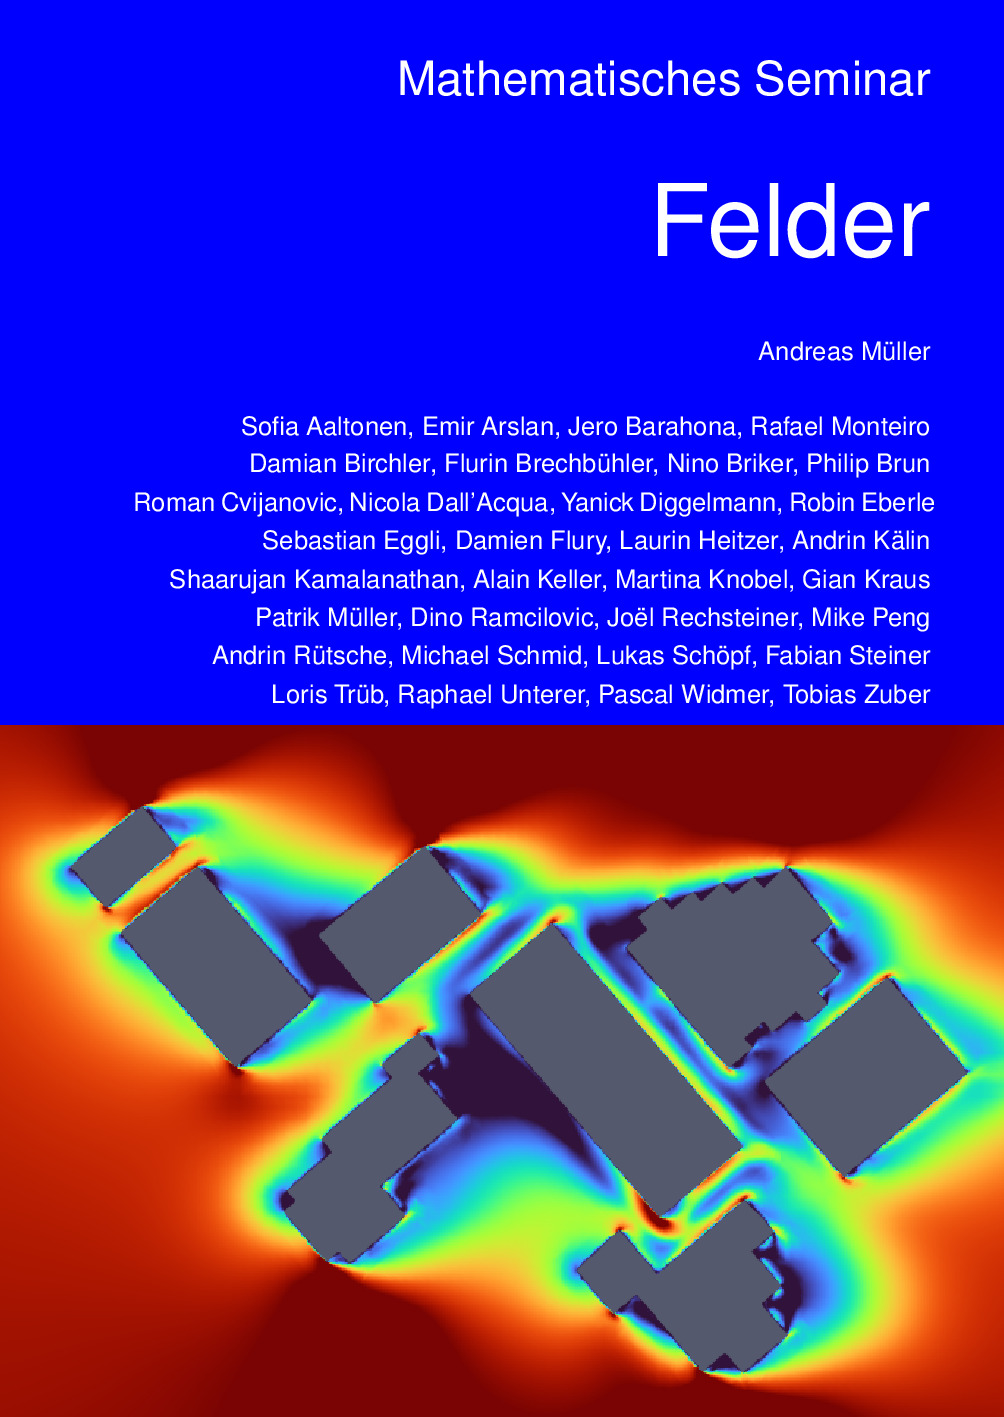
\includepdf{../cover/front.pdf}
\newpage\null\thispagestyle{empty}\newpage
}{}

%
% titlepage.tex
%
\pagestyle{fancy}
\frontmatter
\newcommand\HRule{\noindent\rule{\linewidth}{1.5pt}}
\begin{titlepage}
\vspace*{\stretch{1}}
\HRule
\vspace*{5pt}
\begin{flushright}
{
\LARGE
Mathematisches Seminar\\
\vspace*{20pt}
\Huge
Felder%
}%
\vspace*{5pt}
\end{flushright}
\HRule
\begin{flushright}
\vspace{60pt}
\Large
Leitung: Andreas Müller\\
\vspace{40pt}
\Large
%
% teilnehmer.tex -- Liste der Seminarteilnehmer auf der Titelseite
%
% (c) 2025 Prof Dr Andreas Müller, OST Ostschweizer Fachhochschule
%
Sofia Aaltonen,		% B
Emir Arslan, 		% B
Jero Barahona%,		% E
\\
Ricardo Barbosa,	% B
Damian Birchler,	% EEU
Flurin Brechbühler%,	% E
\\
Nino Briker,		% E
Philip Brun,		% E
Domenico Cardini%,	% EEU
\\
Roman Cvijanovic,	% I
Nicola Dall'Acqua,	% I
Yanick Diggelmann%,	% E
\\
Robin Eberle,		% MSE
Sebastian Eggli,	% EEU
Damien Flury,		% I
Laurin Heitzer%,		% E
\\
Andrin Kälin,		% E
Shaarujan Kamalanathan,	% E
Alain Keller%,		% MSE
\\
Martina Knobel,		% E
Gian Kraus,		% E
Patrik Müller,		% MSE
Joël Rechsteiner%,	% MSE (extern)
\\
Mike Peng,		% E
Andrin Rütsche,		% E
Sagithiya Saseekaran%,	% B
\\
Michael Schmid,		% MSE
Lukas Schöpf,		% MSE
Fabian Steiner,		% E
Loris Trüb%,		% EEU
\\
Raphael Unterer,	% MSE
Pascal Widmer,		% E
Tobias Zuber%,		% M-I
\\

\end{flushright}
\vspace*{\stretch{2}}
\begin{center}
OST Ostschweizer Fachhochschule, Rapperswil, 2025
\end{center}
\end{titlepage}


% add common macros
%
% macros.tex -- some common macro definitions
%
% (c) 2021 Prof Dr Andreas Müller, OST Ostschweizer Fachhochschule
%
\hypersetup{
    linktoc=all,
    linkcolor=blue
}
\newcounter{beispiel}
\newenvironment{beispiele}{
\bgroup\smallskip\parindent0pt\bf Beispiele\egroup

\begin{list}{\arabic{beispiel}.}
  {\usecounter{beispiel}
  \setlength{\labelsep}{5mm}
  \setlength{\rightmargin}{0pt}
}}{\end{list}}
\newcounter{uebungsaufgabezaehler}
% environment fuer uebungsaufgaben
\newenvironment{uebungsaufgaben}{%
}{%
\vfill\pagebreak}
\newenvironment{teilaufgaben}{
\begin{enumerate}
\renewcommand{\theenumi}{\alph{enumi})}
%\renewcommand{\labelenumi}{\alph{enumi})}
\renewcommand{\labelenumi}{\theenumi}
}{\end{enumerate}}
% Aufgabe
\newcounter{problemcounter}[chapter]
\def\aufgabenpath{chapters/uebungsaufgaben/}
\def\ainput#1{\input\aufgabenpath/#1}
\def\verbatimainput#1{\expandafter\verbatiminput{\aufgabenpath/#1}}
\def\aufgabetoplevel#1{%
\expandafter\def\expandafter\inputpath{#1}%
\let\aufgabepath=\inputpath
}
\def\includeagraphics[#1]#2{\expandafter\includegraphics[#1]{\aufgabepath#2}}
% \aufgabe
\renewcommand\theproblemcounter{\thechapter.\arabic{problemcounter}}
\newcommand{\uebungsaufgabe}[1]{%
\refstepcounter{problemcounter}%
\label{#1}%
\bigskip{\parindent0pt\strut}\hbox{\bf\theproblemcounter. }%
\expandafter\def\csname aufgabenpath\endcsname{\inputpath/}%
\expandafter\input{\aufgabenpath/#1.tex}
}
% linsys
\newcolumntype{\linsysR}{>{$}r<{$}}
\newcolumntype{\linsysL}{>{$}l<{$}}
\newcolumntype{\linsysC}{>{$}c<{$}}
\newenvironment{linsys}[1]{%
\begin{tabular}{*{#1}{\linsysR@{\;}\linsysC}@{\;}\linsysR}}%
{\end{tabular}}

% Loesung
\def\swallow#1{
%nothing
}
\NewEnviron{loesung}[1][Lösung]{%
\begin{proof}[#1]%
\renewcommand{\qedsymbol}{$\bigcirc$}
\BODY
\end{proof}
}
\NewEnviron{bewertung}{%
\begin{proof}[Bewertung]%
\renewcommand{\qedsymbol}{}
\BODY
\end{proof}
}
\NewEnviron{diskussion}{%
\begin{proof}[Diskussion]%
\renewcommand{\qedsymbol}{}
\BODY
\end{proof}
}
\NewEnviron{hinweis}{%
\begin{proof}[Hinweis]%
\renewcommand{\qedsymbol}{}
\BODY
\end{proof}
}
\def\keineloesungen{%
\RenewEnviron{loesung}{\relax}
\RenewEnviron{bewertung}{\relax}
\RenewEnviron{diskussion}{\relax}
}
\newenvironment{beispiel}{%
\refstepcounter{satz}
\begin{proof}[Beispiel \arabic{chapter}.\arabic{satz}]%
\renewcommand{\qedsymbol}{$\bigcirc$}
}{\end{proof}}

\allowdisplaybreaks

\lhead{Inhaltsverzeichnis}
\rhead{}
\tableofcontents
\newtheorem{satz}{Satz}[chapter]
\newtheorem{hilfssatz}[satz]{Hilfssatz}
\newtheorem{korollar}[satz]{Korollar}
\newtheorem{lemma}[satz]{Lemma}
\newtheorem{definition}[satz]{Definition}
\newtheorem{annahme}[satz]{Annahme}
\newtheorem{frage}[satz]{Frage}
\newtheorem{problem}[satz]{Problem}
\newtheorem{aufgabe}[satz]{Aufgabe}
\newtheorem{prinzip}[satz]{Prinzip}
\newtheorem*{problem*}{Problem}
\newtheorem{forderung}{Forderung}[chapter]
\newtheorem{konsequenz}[satz]{Konsequenz}
\newtheorem{algorithmus}[satz]{Algorithmus}

% English variants
\newtheorem{theorem}[satz]{Theorem}

\renewcommand{\floatpagefraction}{0.7}

\definecolor{darkgreen}{rgb}{0,0.6,0}
\definecolor{darkred}{rgb}{0.8,0,0}
\definecolor{orange}{rgb}{1,0.6,0}
\definecolor{gelb}{rgb}{1,0.8,0}
%
% Kopfzeilen
%
\fancyfoot{}
\fancyhead{}
%\def\kopfrechts#1{
%\edef\theshortsection{\arabic{section}}
%\rhead{\theshortsection. #1}}
%\def\kopflinks#1{\lhead{\thechapter. #1}
%\rhead{}}
\def\kopfrechts#1{
\global\def\kopfinhalt{#1}
\xdef\theshortsection{\thechapter.\arabic{section}}
\fancyhead[LO]{\theshortsection. #1}}
%
\def\kopflinks#1{
\global\def\kapitelinhalt{#1}
\fancyhead[RE]{\thechapter. #1}
\thispagestyle{empty}
\fancyhead[LO]{}}
% Kapitelautor
\def\chapterauthor#1{{\large #1}\bigskip\bigskip}
%
%
% Uebungsaufgaben
%
\def\uebungsabschnitt{%
\begingroup

\bigskip

\noindent
\vbox to0.3cm{\hbox to\textwidth{\normalfont\large\bfseries Übungsaufgaben}\vfill}
%\keineloesungen%
\nopagebreak%
\fancyhead[RE]{\thechapter. \kapitelinhalt}%
\fancyhead[LE]{\thepage}%
\fancyhead[LO]{Übungsaufgaben}%
\fancyhead[RO]{\thepage}%
\addcontentsline{toc}{section}{Übungsaufgaben}%
}
\def\enduebungsabschnitt{
\endgroup
\bigskip
}
%
\fancyhead[LE]{\thepage}
\fancyhead[RO]{\thepage}
% Transposition
\def\transpose#1{{{#1}^t}}
% Real- und Imaginaerteil
\def\Re{\operatorname{Re}}
\def\Im{\operatorname{Im}}
\def\tr{\operatorname{tr}}
\def\sign{\operatorname{sign}}
\def\grad{\operatorname{grad}}
\def\supp{\operatorname{supp}}%


\mainmatter
%
% part1.tex
%
% (c) 2018 Prof Dr Andreas Müller, Hochschule Rapperswil
%
\begin{refsection}
%
% vorwort.tex -- Vorwort zum Buch zum Seminar
%
% (c) 2019 Prof Dr Andreas Mueller, Hochschule Rapperswil
%
\chapter*{Vorwort}


Dieses Buch entstand im Rahmen des Mathematischen Seminars
im Frühjahrssemester 2025 an der Ostschweizer Fachhochschule in Rapperswil.
Die Teilnehmer, Studierende der Studiengänge für Elektrotechnik, Informatik,
Erneuerbare Energien und Umwelttechnik und Bauingenieurwesen
der OST, erarbeiteten nach einer Einführung in das Themengebiet jeweils
einzelne Aspekte des Gebietes in Form einer Seminararbeit, über
deren Resultate sie auch in einem Vortrag informierten. 

Im Frühjahr 2025 waren Felder das Thema des Seminars.

In einigen Arbeiten wurde auch Code zur Demonstration der 
besprochenen Methoden und Resultate geschrieben, soweit
möglich und sinnvoll wurde dieser Code im Github-Repository
\index{Github-Repository}%
dieses Kurses%
\footnote{\url{https://github.com/AndreasFMueller/SeminarFelder.git}}
\cite{buch:repo}
abgelegt.
Im genannten Repository findet sich auch der Source-Code dieses
Skriptes, es wird hier unter einer Creative Commons Lizenz
zur Verfügung gestellt.


\part{Grundlagen}

%
% chapter.tex -- Kapitel 3: 1-Formen und Kurvenintegrale
%
% (c) 2024 Prof Dr Andreas Müller
%
\chapter{Differentialformen und Kurvenintegrale
\label{chapter:kurvenintegral}}
\kopflinks{Differentialformen und Kurvenintegrale}

\noindent
Ein Flug zum Mars muss Energie aufwenden, um gegen die Schwerkraft der
Sonne von der Erdbahn aus zur Entfernung des Mars von der Sonne zu
gewinnen.
\index{Mars}%
\index{Erdbahn}%
In der Praxis wird dies dadurch erreicht, dass man dem Raumfahrzeug
mithilfe von Raketentriebwerken genügend kinetische Energie erteilt.
\index{Raumfahrzeug}%
\index{Rakete}%
Es folgt dann einer elliptischen Bahn, die ihren sonnenfernsten Punkt
bei der Marsbahn hat.
\index{Bahn!elliptisch}%
\index{elliptische Bahn}%
Während des Fluges wird laufend kinetische Energie des Raumschiffs in
potenzielle Energie umgewandelt werden.
Mit jedem kleinen Teilstück der Flugbahn verliert das Raumschiff 
kinetische Energie, die proportional ist zur Kraftkomponente parallel
zur Flugbahn. 
Das potentielle Energiepaket, das während des Teilstücks gewonnen wird,
ist linear vom Tangentialvektor der Bahn abhängig.
Die gesamte potentielle Energie, die zwischen Erde und Marsbahn
gewonnen wird, ist die Summe dieser Teilstücke.
Mathematisch wird es durch eine Art Integral einer Funktion dargestellt,
welches sowohl linear von der Bahntangente wie auch vom Pfad des
Raumschiffs abhängt.
Diese Integralkonstruktion muss aber so erfolgen, dass Sie nicht von der
Wahl von Koordinatensystemen und Parametrisierungen abhängt, was in
diesem Kapitel durchgeführt werden soll.
Sie muss ausserdem so funktionieren, dass sie sich über mehrer
Koordinatensysteme hinweg zusammensetzen lässt, wie dies bei einer
Bahn auf einer Mannifaltigkeit unvermeidlich wird.

%
% 1-Formen
%
\section{1-Formen}
Was ist es eigentlich, was man integrieren will?
Zunächst gibt der riemannsche Integralbegriff aus dem elementaren
Analysisunterricht den Eindruck, dass es eine Funktion ist.
Es können aber nicht allein die Funktionswerte sein, die das Integral
bestimmen.
Vielmehr kommt es auch darauf an, wie ``schnell'' der Definitionsbereich
beim Integrieren durchlaufen wird.
Dies wird zum Beispiel durch die Substitutionsformel für das Integral
wiedergegeben.
Man kann sie auch als eine Koordinatenänderungsformel für das Integral
entlang der reellen Achse betrachten.
Was ist dann aber die koordinatenunabhängige Grösse, deren Integral
bestimmt worden ist?
Dies soll in diesem Abschnitt geklärt werden.

%
% Riemann-Integral
%
\subsection{Riemann-Integral}
Im elementaren Analysis-Unterricht lernt man, dass das Riemann-Integral
\[
I
=
\int_a^b f(x)\,dx
\]
einer Funktion $f(x)$ die Fläche unter der Kurve $y=f(x)$ berechnet.
Man macht das, indem man die Fläche in zunächst in vertikale Streifen
der Breite $\Delta x_i$ zerlegt, die an bei den Koordinaten $x_i$
beginnen.
Die Rechtecke dürfen sich nicht überlappen und müssen die Fläche unter
der Kurve vollständig abdecken, die Teilstellen $x_i$ müssen
also $x_{i+1}=x_i+\Delta x_i$ erfüllen.
Dann ist die Summe
\begin{equation}
\sum_{i} f(x_i)\cdot \Delta x_i
\approx 
I
\label{buch:kurvenintegral:1-form:eqn:riemann-summe}
\end{equation}
eine Approximation für den Wert des Riemann-Integrals.

Der Unterschied zum exakten Wert kommt vor allem daher, dass die
Rechtecke mit Breite $\Delta x_i$ und Höhe $f(x_i)$ manchmal
die Funktionskurve überragen, zum Beispiel wenn die Kurve negative
Steigung hat, und manchmal darunter bleiben, wenn die Kurve positive
Steigung hat.
Der Unterschied setzt sich aus Dreiecken zusammen, deren Grundseite
$\Delta x_i$ ist, und deren Höhe durch $f'(x_i)\cdot \Delta x_i$
beschränkt ist.
Der Fehler ist daher grössenordnungsmässig nicht grösser als
\[
\Delta I
\approx
\sum_i \Delta x_i \cdot |f'(x_i)\cdot \Delta x_i|
=
\sum_i |f'(x_i)| \Delta x_i^2.
\]
Sorgt man dafür, dass die Schritte $\Delta x_i$ alle gleich klein
sind, also $\Delta x_i=h$, dann folgt
\[
\Delta I
\approx
\sum_i |f'(x_i)| h^2
=
h\sum_i |f'(x_i)|h
\approx
h\int_a^b |f'(x)|\,dx.
\]
Für eine stetig differenzierbare Funktion ist $f'(x)$ im Integranden
auf der rechten Seite beschränkt.
Das Integral auf der rechten Seite ist also beschränkt.
Es bleibt aber der Faktor $h$, der den Fehler $\Delta I$ beliebig
klein macht, wenn man $h$ gegen $0$ gehen lässt.

%
% Substitution
%
\subsection{Substitution}
Der Integrand $f(x)$ im Riemann-Integral ist offenbar eine von
der Parametrisierung unabhängige Grösse.
Wechselt man die Koordinaten mit Hilfe einer Koordinatentransformation
$x(y)$, dann bleiben die Werte $f(x(y))$ an entsprechenden Stellen
des Definitionsbereiches die gleichen.
Es ändert sich aber das durch den Faktor $dx$ im Integral symbolisierte
Gewicht, mit dem jeder Summand in der Riemann-Summe
\eqref{buch:kurvenintegral:1-form:eqn:riemann-summe}
gewichtet wird.
Die Koordinatentransformation $x(y)$ macht aus einem Schritt $\Delta y$
einen $x$-Schritt von der Grössenordnung
\[
\Delta x
\approx
\frac{dx}{dy}(y)\cdot \Delta y.
\]
Sind $a'$ und $b'$ die Endpunkte des $y$-Intervalls, die auf 
$a=x(a')$ und $b=x(b')$ abgebildet werden, dann ist daher das
Integral
\begin{equation}
\int_a^b f(x)\,dx
=
\int_{a'}^{b'} f(x(y)) \, \frac{dx}{dy}(y)\,dy.
\label{buch:kurvenintegral:1-form:eqn:substitution}
\end{equation}
Dies ist die bekannt Formel für die Substitutionsformel für das Integral.


%
% Integral über ein eindimensionales Definitionsgebiet
%
\subsection{Integral über ein eindimensionales Definitionsgebiet
\label{buch:1formen:subsection:integral}}
\input{chapters/030-kurvenintegral/fig/fig-1koordinaten.tex}
Die Substitutionsformel erklärt, wie das Integral angepasst werden
muss, wenn man von einer Koordinatenwahl $x$ zur alternativen
Koordinate $y$ wechseln will.
Wir können das Integral aber auch als eine Zahl betrachten,
die nur von zwei rein geometrisch definierten Eigenschaften
abhängig sind.
Einerseits ist dies eine Teilmenge eines eindimensionalen
Definitionsgebietes, welches in
Abbildung~\ref{buch:kurvenintegral:fig:1koordinaten} durch
den Bereich zwischen den Punkten $A$ und $B$ entlang der Menge $M$
symbolisiert ist.
Durch die Koordinatenssysteme $\varphi$ und $\psi$ werden daraus
die Intervalle $[a,b]$ von $x^1$-Koordinatenwerten bzw.~$[a',b']$
von $y^1$-Koordinatenwerten.

Die zweite Komponente zur Definition des Integrals ist eine
noch zu definierende Grösse $\alpha$, die die Funktionswerte
entlang des Definitionsgebietes liefert.
Dies muss so geschehen, dass $\alpha$ wieder ein Objekt ist,
welches vom Koordinatensystem unabhängig definiert ist, oder 
besser, dessen Transformationseigenschaften beim Koordinatenwechsel
klar sind.
Als Leitlinie für die gesuchte Umrechnungsformel kann die
Substitutionsformel
\eqref{buch:kurvenintegral:1-form:eqn:substitution}
herangezogen werden.

Das gesamte Integral möchten wir als
\[
\int_{AB} \alpha
\]
schreiben können.
Es soll die üblichen Eigenschaften eines Integrals haben, also
insbesondere linear sein:
\[
\int_{AB}
(\alpha + \beta)
=
\int_{AB}
\alpha
+
\int_{AB}
\beta
\qquad\text{und}\qquad
\int_{AB}
t
\alpha
=
t
\int_{AB}
\alpha.
\]
In einem Koordinatensystem soll eine Integralformel entstehen.
Rein formal ist daher $\alpha$ in den Koordinatensystemen $\varphi$
bzw.~$\psi$ durch
\[
f(x^1)\,dx^1
\qquad
\text{bzw.}
\qquad
g(y^1)\,dy^1
\]
gegeben.
Die Substitutionsformel
\eqref{buch:kurvenintegral:1-form:eqn:substitution}
besagt dann, dass
\[
g(y^1)
= 
f(\varphi\circ\psi^{-1}(y^1))
\frac{dx^1}{dy^1}(y^1)
=
f(\varphi\circ\psi^{-1}(y^1))
\frac{d}{dy^1}(\varphi\circ\psi^{-1}(y^1))
\]
sein muss.
Man beachte, dass $g(y^1)$ und $f(x^1)$ nicht Komponenten eines
Vektors sind, dann für Vektorkomponenten $v_1$ gilt wegen
\[
\frac{\partial}{\partial y^1}
=
\frac{dx^1}{\partial y^1}\cdot \frac{\partial }{\partial x^1}.
\]
die Umrechnungsformel
\[
v_1'(y^1)
=
\frac{dy^1}{dx^1}
v_1(x^1)
\qquad\text{oder}\qquad
v_1(x^1)
=
\frac{dx^1}{dy^1} v_1'(y^1).
\]
Die Transformation erfolgt also in der ``falschen'' Richtung.

Aus der Sicht des angestrebten Ziels, ein koordinatenunabhängiges
Integralkonzept zu definieren, ist die gegenüber Vektoren ``verkehrte''
Transformationsrichtung zu erwarten.
Wenn ein Koordinatenwechsel dazu führt, dass der Koordinatenraum
langsamer durchlaufen wird, äussert sich das darin, dass die Komponenten
eines Tangentialvektors grösser werden.
Der Tangentialvektor beschreibt aber die ``Schrittgrösse $dx$'' beim
Integrieren auf koordinatenunabhängige Art.
Damit das Integral gleich bleibt, muss der skalare Faktor entsprechend
kleiner werden.

%
% Transformation von Linearformen
%
\subsection{Linearformen
\label{buch:kurvenintegral:1formen:subsection:linearformen}}
Die im vorangegangenen Abschnitt heuristisch hergeleitete
Transformationseigenschaft ist nicht so überraschend, man kann sie
auch in der linearen Algebra bei Linearformen finden.
In diesem Abschnitt soll die Koordinatentransformationsregel für
Linearformen formuliert werden.

%
% Koeffizienten einer Linearform
%
\subsubsection{Koeffizienten einer Linearform}
Seien $a^i$ die Komponenten eines Vektors $a$ in einer Basis $e_i$ und
$t_{i}\mathstrut ^k$ die Koeffizienten der Transformationsmatris
in eine alternative Basis $e'_k$.
Die Komponenten in der alternativen Basis werden mit $a^{\prime k}$
bezeichnet und die Umrechung zwischen den Koordinaten erfolgt mit der
Formel
\begin{equation}
a^{\prime k}
=
t^k\mathstrut_i a^i
\label{buch:kurvenintegral:1formen:linearformen:vektor}
\end{equation}
gegeben.

Eine Linearform ist eine lineare Abbildung $l\colon V\to\mathbb{R}$,
die einem Vektor $v$ einen Zahlenwert $l(v)$ zuordnet.
Die Linearität verlangt, dass der Wert
\[
l(a)
=
\sum_i
l(a^ie_i)
=
a^i \underbrace{l(e_i)}_{\displaystyle=l_i}
\]
ist (man beachte die einsteinsche Summationskonvention).
Die Werte $l_i=l(e_i)$ sind die Koeffizienten, mit denen die $a^i$
multipliziert werden müssen, um $l(a)$ zu ergeben.
Entsprechend sind die $l'_i=l(e'_i)$ die Koeffizienten der Basis

%
% Transformation der Koeffizienten einer Linearform
%
\subsubsection{Transformation der Koeffizienten einer Linearform}
Bei der Koordinatentransformation soll sich der Wert $l(a)$ nicht
ändern, es muss daher
\[
l(a)
=
l'_k
a'^k
=
l'_k
(t^k\mathstrut _i a^i)
=
(l'_kt^k\mathstrut_i) a^i
=
l_i
a^i
\]
sein.
Da dies für jeden beliebigen Vektor gelten muss, müssen die Koeffizienten
übereinstimmen und es folgt das Transformationsgesetz
\begin{equation}
l'_kt^k\mathstrut_i
=
l_i
\label{buch:kurvenintegral:1formen:linearformen:linearform}
\end{equation}
für die Koeffizienten der Linearform.
Die Transformation der Linearformkoeffizienten erfolgt also
in der umgekehrten Richtung vom gestrichenen Koordinatensystem 
zum ungestrichenen.
Ausserdem wird über den obneren Index von summiert statt über
den unteren wie in 
\eqref{buch:kurvenintegral:1formen:linearformen:vektor}.

Betrachtet man die Koeffizienten $t^k\mathstrut_i$ als Matrix, mit der
die Umrechnung der Koeffizienten von $a$ erfolgt, dann ist die Matrix,
mit der die Koeffizienten $l_k'$ umberechnet werden, die transponierte
Matrix.

%
% Linearformen als Zeilenvektoren
%
\subsubsection{Linearformen als Zeilenvektoren}
Der Wert einer Linearform $l$ auf einem Vektor $a$ kann in Komponenten
als
\[
l(a) = \sum_{i=1}^n l_ia^i
\]
geschrieben werden.
In der Matrixform
\[
l(a)
=
\begin{pmatrix}l_1&\dots&l_n\end{pmatrix}
\begin{pmatrix}
a^1\\[-2pt]
\vdots\\
a^n
\end{pmatrix}
\]
zeigt sich, dass Linearformen als Zeilenvektoren betrachtet werden
sollten.

Das Transformationsgesetz
\eqref{buch:kurvenintegral:1formen:linearformen:linearform}
für Linearformen bestätigt dies.
Schreibt man das Transformationsgesetz für die Komponenten des
Vektors mit den Koeffizienten als
\[
a^{\prime i}
=
\sum_{k=1}^n t^i\mathstrut_k a^i
\]
und berechnet den Wert $l(a)$ in Koordinaten als
\[
l(a)
=
\sum_{i=1}^n l'_i a^{\prime i}
=
\sum_{i=1}^n
l'_i
\sum_{k=1}^n
t^i\mathstrut_k a^k
=
\sum_{k=1}^n
\biggl(
\sum_{i=1}^n
l'_i
t^i\mathstrut_k
\biggl)
a^k
=
\sum_{k=1}^n
l_k
a^k.
\]
Man liest also ab, dass die Koeffizienten der Normalform nach dem
Gesetz
\[
l_k
=
\sum_{i=1}^n
l'_i
t^i\mathstrut_k
\]
transformiert werden.
In Matrixform geschrieben bedeutet dies
\[
\begin{pmatrix}l_1&\dots&l_n\end{pmatrix}
=
\begin{pmatrix}l_1'&\dots&l_n'\end{pmatrix}
\begin{pmatrix}
t^1\mathstrut_1 & \dots  & t^1\mathstrut_n \\[-3pt]
\vdots          & \ddots & \vdots          \\
t^n\mathstrut_1 & \dots  & t^n\mathstrut_n
\end{pmatrix}.
\]
Die Transformation erfolgt also mit der gleichen Matrix, aber
einerseits durch Multiplikation des Zeilenvektors von rechts
und vor allem in der umgekehrten Richtung von den gestrichtenen
zu den ungestrichenen Koordinaten:
\[
l = l' T
\qquad\Rightarrow\qquad l' = lT^{-1}.
\]

%
% Kovariante und kontravariante Indizes
%
\subsubsection{Kovariante und kontravariante Indizes}
Die Koeffizienten einer Linearform und die Komponenten eines Vektors 
haben also entgegengesetztes Transformationsverhalten.
Es können die gleichen Koeffizienten der Transformationsmatrix 
verwendet werden, aber die Transformation erfolgt in der umgekehrten
Richtung und es muss über den anderen Index summiert werden.
Das unterschiedliche Verhalten wurde bereits durch die unterschiedliche
Position der Indizes vorweggenommen.
Während Vektorkomponenten obere Indizes verwenden, haben die
Koeffizienten einer Linearform untere Indizes.

\begin{definition}[kovariant und kontravariant]
Die Komponenten eines Vektors heissen {\em kontravariant}, sie haben
\index{kontravariant}%
einen hochgestellten Index, der ebenfalls {\em kontravariant} genannt
wird.
Die Koeffizienten einer Linearform von Vektoren heissen dargegen
{\em kovariant}, sie tragen einen unteren Index, der entsprechend
\index{kovariant}%
{\em kovariant} genannt wird.
\end{definition}

%
% Tensoren
%
\subsubsection{Tensoren}
Wir werden später sehen, dass es sinnvoll sei kann, dass eine Grösse
mehr als einen Index haben kann.
Zum Beispiel hängt die Kraft auf eine bewegte Ladung linear von der
Richtung des Magnetfeldes und von der aktuellen Bewegungsrichtung ab.
Beide Einflussfaktoren haben vektoriellen Charakter, werden also durch
Komponenten beschrieben, die ihrerseits verschiedene Komponenten haben.
Daher vereinheitlichen und verallgemeinern wir die Konzepte von Vektoren
und Linearformen zum neuen Begriff des Tensors.

Als etwas konkreteres Beispiel betrachten wir das Skalarprodukt von
zwei Vektoren $u$ und $v$ mit den Komponenten $u^i$ bzw.~$v^k$.
In der Vektorgeometrie lernt man, dass man das Skalarprodukt mit der
Formel $\sum_i u^iv^i$ berechnen kann.
Man lernt aber auch, dass diese einfache Formel nur für in einem
orthonormierten Koordinatensystem gilt, wo die Basisvektoren
orthogonal sind und Länge $1$ haben.
Insbesondere ist die angegebene Formel für das Skalarprodukt nicht
für beliebige Koordinatensysteme tauglich.

Schreibt man die Vektoren $u$ und $v$ explizit als Linearkombinationen
\[
u = \sum_{i=1}^n u^i b_i
\qquad\text{und}\qquad
v = \sum_{k=1}^n v^k b_k
\]
der Basisvektoren, dann ist das Skalarprodukt durch
\[
u\cdot v
=
\sum_{i,k=1}^n u^iv^k \underbrace{(b_i\cdot b_k)}_{\displaystyle g_{ik}}
\]
gegeben.
Für eine orthonormierte Basis sind die Koeffizienten
\[
g_{ik}
=
\left\{
\begin{array}{llcl}
1&\quad i=k&\qquad\Leftrightarrow\qquad&\text{Basisvektor $b_i$ hat Länge $|b_i|=1$}\\
0&\quad i\ne k&\qquad\Leftrightarrow\qquad&\text{Basisvektoren $b_i$ und $b_k$ sind orthogonal: $b_i\perp b_k$}
\end{array}
\right.
\]
Für beliebige Koordinatensysteme muss aber zugelassen werden, dass 
die Koeffizienten $g_{ik}$ beliebige Werte annehmen können.

\begin{definition}[metrischer Tensor]
Die Koeffizienten $g_{ik}$, die das Skalarprodukt zweier Vektoren durch
\[
u\cdot v
=
\sum_{i,k=1}^n u^iv^k g_{ik}
\]
heisst der {\em metrische Tensor}.
\index{metrischer Tensor}%
\end{definition}

Der metrische Tensor hat interessante zusätzliche Eigenschaften.
Er ist zum Beispiel symmetrisch, was sich in $g_{ik}=g_{ki}$ für
alle Paare $i,k$ äussert.
Ausserdem ist das Skalarprodukt üblicherweise positiv definit,
so dass 
\[
g_{ik}u^i u^k
>
0
\]
für von $0$ verschiedene Vektoren $u$ gilt.

Der metrische Tensor definiert das Skalarprodukt, welches eine bilineare
Abbildung ist, die aus zwei Vektoren auf jeweils lineare Art einen
Zahlenwert berechnet.
Man kann ihn aber auch anders interpretieren.
Gibt man nur einen Vektor mit den Komponenten $v^i$ vor, erzeugt der
metrische Tensor eine Linearform mit den Koeffizienten
\[
l_k = g_{ki}v^i
\]
Die Komponenten $l_k$ kann man auch ermitteln, indem man das Skalar
von $v$ mit den Basisvektoren berechnet.
Man kann also die Indizes des metrischen Tensors als Indizes betrachten,
die mit einem Inputvektor verknüpft werden, oder alternativ als Indizes
der Komponenten der Output-Linearform.

Es ist auch denkbar, anstelle von Vektoren aus Linearformen
neue Werte zu berechnen, oder mehr als zwei Faktoren einfliessen zu
lassen.
Zum Beispiel kann die Krümmung des Raumes dadurch beschrieben werden,
dass der Transport eines Vektors (erster Inputvektor) beim Paralleltransport
entlang eines Parallelogramms (zwei weitere Inputvektoren) gedreht wird.
Die Krümmung berechnet also auf lineare Weise aus drei Inputvektoren
einen Outputvektor.

\begin{definition}[Tensor]
\index{Tensor}
Ein {\em Tensor $r$-ter Stufe} ist eine multilineare Abbildung, die
$r$ Vektoren oder Linearformen auf Skalare abbildet.
Seine Komponenten sind durch eine Grösse
$A^{i_1\dots i_k}\mathstrut_{i_{k+1}\dots i_r}$
mit $r$ Indizes gegeben.
Der Tensor heisst vom Typ $(k,r-k)$ wenn er $k$ kovariante und 
$r-k$ kontravariante Indizes hat.
\end{definition}

Ein Skalar ist ein Tensor nullter Stufe.
Ein Vektor ist ein Tensor erster Stufe mit einem kontravarianten Index,
also vom Typ $(0,1)$, während eine Linearform ein Tensor erster
Stufe vom Type $(0,1)$ ist.
Der metrische Tensor $g_{ik}$ ist ein Tensor zweiter Stufe vom Typ
$(2,0)$.
Ein Tensor vom Typ $(1,1)$ hat Komponenten $a^i\mathstrut_k$, die aus
einem Vektor $u^k$ den Vektor mit den Komponenten
\[
v^i = a^i\mathstrut_k u^k
\]
berechnet.
Dies entspricht der Idee einer Matrix, die Vektoren auf andere 
Vektoren abbildet und die man in der linearen Algebra kennenlernt.

Beim metrischen Tensor sind die beiden Indizes wegen der Symmetrie
vertauschbar.
Man beachte aber, dass die Platzierung der Indizes im Allgemeinen nicht
beliebig ist.
Zum Beispiel wird der Riemannsche Krümmungstensor oft in der Form
\(
R^i\mathstrut_{klr}
\)
als Tensor vierter Stufe vom Typ $(3,0)$ geschrieben.
Er ist antisymmetrisch in den letzten beiden Indizes, es gilt also
\(
R^i\mathstrut_{klr}
=
-
R^i\mathstrut_{krl}
\),
es gibt aber keine offensichtlichen weiteren Symmetrien.
Wendet man den Tensor auf zwei Vektoren mit Komponenten $u^l$ und
$v^r$ an, erhält man
\[
a^i\mathstrut_k
=
R^i\mathstrut_{klr}u^lv^r,
\]
worin nur noch die zwei Indizes $i$ und $k$ frei sind.
Der Tensor $a^i\mathstrut_k$ zweiter Stufe vom Typ $(1,1)$
kann als eine Abbildungsmatrix betrachtet werden,
die einen Vektor auf einen anderen Vektoren abbildet.

Da die einsteinsche Summationskonvention nur über verschieden platzierte
Indizes summiert, wird sichergestellt, dass Linearformen nur auf
Vektorkomponenten angewendet werden können.
Da die Transformationsmatrix einen oberen und einen unteren Index hat,
kann sie aus einem kontravarianten Vektor nur wieder einen kontrvarianten
Vektor machen.
Ebenso wird ein kovarianter Index durch Transformation wieder zu einem
kovarianten Index.

%
% Tensoren sind nicht nur Matrizen mit mehr Dimensionen
%
\subsubsection{Tensoren sind nicht nur Matrizen mit mehr Dimensionen}
Auf den ersten Blick besteht eine grosse Ähnlichkeit zwischen dem
Konzept der Matrix und einem Tensor zweiter Stufe.
In der linearen Algebra schreibt man eine lineare Abbildung in einer
Basis durch eine Matrix.
Die Komponenten $u_k$ eines Vektors $u$ werden von der Matrix $A$
mit den Einträgen $a_{ik}$ durch
\[
v = Au
\qquad\Leftrightarrow\qquad
v_i = \sum_{k=1}^n a_{ik}u_k
\]
auf einen Vektor $v$ abgebildet.
Der erste Index, der Zeilenindex, bezeichnet die Komponente, die berechnet
wird, während über den zweiten Index summiert wird.
Ein Matrix wird meistens als rechteckiges Zahlenschema
\[
A
=
\begin{pmatrix}
a_{11} & a_{12} & \dots  & a_{1n} \\
a_{21} & a_{22} & \dots  & a_{2n} \\[-2pt]
\vdots & \vdots & \ddots & \vdots \\[-1pt]
a_{m1} & a_{m2} & \dots  & a_{mn}
\end{pmatrix}
\]
dargestellt.
Die Wirkung einer Matrix auf einem Vektor wird durch das Produkt
``Zeile mal Spalte'' gegeben, summiert wird immer über den zweiten
Index,, den Spaltenindex.

Tensoren erweitern diese Idee in mehrfacher Hinsicht.
Zunächst wird die Möglichkeit zusätzlicher Indizes geschaffen.
Man könnte die Koeffizienten als drei- oder noch höherdimensionales
Zahlenschema darstellen.
Allerdings ist dies auch nicht weiter hilfreich für die zweite
Erweiterung: jeder Index kann als Summationsindex verwendet werden.

In der Matrizenrechnung wird kein Unterschied zwischen kovarianten
und kontravarianten Indizes gemacht.
Es ist durchaus üblich, die Koeffizienten $g_{ik}$ des metrischen
Tensors als Einträge einer Matrix zu betrachten.
Sie wird die {\em Gram-Matrix} genannt und kann dazu verwendet
\index{Gram-Matrix}T
werden, das Skalarprodukt als 
\[
u\cdot v
=
u^t G v
=
\sum_{i,k=1}^n
g_{ik}u_iv_k
\]
zu schreiben.
Allerdings sind die Koeffizienten
\[
\sum_{k=1}^n a_{ik}u_k
\qquad\text{und}\qquad
\sum_{k=1}^n g_{ik}v_k
\]
für die Abbildungsmatrix bzw.~den metrischen Tensor von ganz verschiedenem
Charakter.
Im ersten Fall entstehen Komponenten eines Vektors, die sich bei Basiswechsel
kontravariant transformieren, im zweiten Fall entstehen Koeffizienten
einer Linearform, die sich kovariant transformieren.
Die bisherige Entwicklung hat aber gezeigt, dass diese Unterscheidung
wesentlich ist, wenn man dem Ziel einer koordinatenunabhängigen
Beschreibung von Naturgesetzen näher kommen will.

%
% Integrand $\alpha$ als Linearform
%
\subsubsection{Integrand $\alpha$ als Linearform}
Der Integrand eines koordinatenunabhängig definirten Integrals entlang
eines eindimensionalen Definitionsgebietes muss also eine
Linearform sind.
Tatsächlich wird das Arbeitsintegral in der Physik definiert als
das Wegintegral der Kraft entlang eines Weges definiert.
Darin wird die Kraft skalar mit dem Tangentialvektor multipliziert
und integriert.
Wir haben das Skalarprodukt bereits durch den metrischen Tensor
beschrieben.
Aus dem Kraftvektor mit den Komponenten $F^k$ macht er die Linearform
mit den Koeffizienten $g_{ik}F^i$.

Solche Linearformen werden auch als $1$-Formen bezeichnet.
Wir werden für Integranden über Gebiete höherer Dimension weitere

%
% Die Koordinaten-1-Formen
%
\subsection{Die Koordinaten-1-Formen}
Ein spezieller Fall tritt ein, wenn der Koeffizient der Integranden-1-Form
$\alpha$ die Zahl $1$ ist.
In diesem Koordinatensystem wird das Integral
\[
\int_{AB} \alpha
=
\int_{a}^{b} 1\, dx^1
=
\int_{a}^b\,dx^1
=
\bigl[ x^1 \bigr]_a^b
=
b-a.
\]
Im $y^1$-Koordinatensystem ist hat das Integral dagegen den Wert
\begin{equation}
\int_{AB}\alpha
=
\int_{a'}^{b'} \frac{dx^1}{dy^1}\,dy^1
=
\bigl[x^1(y^1)\bigr]_{a'}^{b'}
=
x^1(b') - x^1(a')
=
b-a,
\label{buch:kurvenintegral:1formen:eqn:hauptsatz}
\end{equation}
wobei im zweiten Schritt verwendet wurde, dass der Integrand die
Ableitung der Funktion $x^1(y^1)$ nach der Integrationsvariable ist.
Die Funktion $x^1(y^1)$ ist daher die
Stammfunktion des Integranden im zweiten Integral ist.
Wie erwartet, stimmen die Integrale überein.

Die Symbole $dx^1$ und $dy^1$ können daher genauso als Basislinearformen
betrachtet werden, wie die Ableitungsoperatoren
$\partial/\partial x^1$ und $\partial/\partial y^1$ als
Basisvektoren für die Tangentialvektoren betrachtet wurden.
Sie heissen die Koordinaten-1-Formen und sind besonders einfach
zu integrieren.

Eine $1$-Form $\alpha$ hat in einer Dimension die Form
\[
\alpha
=
f(x^1) \,dx^1
\]
und ihr Integral über das Intervall zwischen $A$ und $B$ ist
\[
\int_{AB}\alpha
=
\int_a^b f(x^1)\,dx^1.
\]
Die Notation ist so gewählt, dass sich die neue Betrachtungsweise als
Integral einer 1-Form über ein eindimensionales Gebiet nach Einführung
eines Koordinatensystems mit der konventionellen Riemann-Integration
deckt.

Das Resultat
\eqref{buch:kurvenintegral:fig:1koordinaten}
ist auch als der Hauptsatz der Infinitesimalrechnung bekannt.
Wir halten jedoch fest, dass es von einer Form ist, der wir später
wiederholt begegnen werden.
Das Integral der Ableitung einer Funktion über ein Intervall hat einen
Wert, der nur von den Werten der Funktion auf dem Rand des Intervalls
bestimmt ist.
Der Satz von Stokes wird später zeigen, dass dies ein allgemeines
Phänomen ist.
Das Integral einer geeignet definierten Ableitung eines Integranden
ist bestimmt durch die Werte auf dem Rand des Integrationsgebietes.
Dazu muss aber zunächst die Klasse der möglichen Integranden von
$1$-Formen auf $p$-Formen ausgweitet werden und es muss eine Ableitung
für $p$-Formen konstruiert werden.
Dies wird in den nachfolgenden Abschnitten und Kapiteln geschehen.


%
% Kurvenintegral einer 1-Form
%
\section{Kurvenintegral einer 1-Form
\label{buch:kurvenintegral:section:1form}}
\kopfrechts{Kurvenintegral einer 1-Form}%
Eine Kurve ist eine eindimensionale Untermannigfaltigkeit in
einer $n$-dimensionalen Mannigfaltigkeit $M$.
Eine $1$-Form auf der Mannigfaltigkeit $M$ führt zu einer 
$1$-Form auf der Kurve und damit wird es möglich, das Integral
dieser 1-Form auf der Kurve zu berechnen.
Dies soll in diesem Abschnitt schrittweise durchgeführt werden.

%
% 1-Form auf einer Mannigfaltigkeit
%
\subsection{$1$-Form auf einer Mannigfaltigkeit}
Eine $1$-Form auf einer $n$-dimensionalen Mannigfaltigkeit ist eine
Linearform, die auf einen Tangentialvektor angewendet werden kann
und einen Zahlenwert ergibt.
In einem Koordinatensystem mit den Koordinaten $x^1,\dots,x^n$ bilden
die Tangentialvektoren an die Koordinatenlinien eine Basis des
Tangentialraumes.
Die einzelnen Basisvektoren sind früher schon mit den
Ableitungsoperatoren $\partial/\partial x^i$ identifiziert worden.
Die Koordinaten-1-Formen $dx^1,\dots,dx^n$ ermitteln, wie schnell sich
die entsprechende Koordinate entlang eines Tangentialvektors ändert.
Da sich entlang einer Koordinatenlinie immer nur eine einzige
Koordinate ändert, gilt
\[
\biggl\langle dx^i,\frac{\partial}{\partial x^k}\biggr\rangle
=
\delta_{ik}
=
\begin{cases}
1&\qquad \text{falls $i=k$}\\
0&\qquad \text{sonst}.
\end{cases}
\]
\index{<,>@$\langle\;,\;\rangle$}%
Man nennt diese Basis der Linearformen auch die zur Basis der
Ableitungsoperatoren \emph{duale Basis}.

Eine $1$-Form auf der Mannigfaltigkeit hat daher im Koordinatensystem
mit den Koordinaten $x^i$ die Form
\[
\alpha
=
\alpha_i(x)\, dx^i,
\]
wobei wieder die Summationskonvention gilt.

\begin{beispiel}
Die $1$-Form
\[
\beta
=
-
\sum_{i=1}^n
\frac{GMx^i}{r^3}
dx^i
\]
soll auf dem Impulsvektor eines Teilchens berechnet werden.
Die Summationskonvention ist hier nicht anwendbar, da der Index $i$ zweimal
als oberer Index auftritt.
\index{Impuls}%
Wird die Bahnkurve mit der Zeit parametrisiert, hat der Geschwindigkeitsvektor
die Komponenten $\dot{x}^i$.
Der Impuls $p$ des Teilchens ist der Vektor mit den Komponenten
$p^i=m\dot{x}^i$.
Wendet man die Linearform $\beta$ darauf an, ergibt sich
\begin{align}
\langle \alpha, p\rangle
&=
-
\frac{GMm}{r^3}
\biggl\langle \sum_i x^i\,dx^i, \sum_k\dot{x}^k\frac{\partial}{\partial x_k}\biggr\rangle
=
-
\frac{GMm}{r^3}
\sum_{i,k} x^i \biggl\langle dx^i,\dot{x}^k\frac{\partial}{\partial x_k}\biggr\rangle
\notag
\\
&=
-
\frac{GMm}{r^3}
\sum_{i,k}
x^i \delta_{ik} \dot{x}^k
=
-\frac{GMm}{r^3}
\sum_i x^i\dot{x}^i
\label{buch:kurvenintegral:kurvenintegral:eqn:gravimpuls}
\end{align}
Dies ist die Leistung, die das Teilchen gegen das Gravitationsfeld 
arbeitet.
Eine $1$-Form ist also dazu geeignet, ein wichtiges physikalisches Konzept
des Gravitationsfeldes auszudrücken.
\end{beispiel}

Die Form
\eqref{buch:kurvenintegral:kurvenintegral:eqn:gravimpuls}
ist allerdings noch nicht wirklich geeignet.
In der Formel wurden kontravariante Komponenten miteinander multipliziert
und summiert, dies führt nicht auf eine koordinatensystemunabhängige
Grösse.
Dazu müssten aus einem oberen Index in unterer gemacht werden können
oder umgekehrt.
Mit einer Metrik ist dies möglich, wie die musikalischen Operationen
gemäss
Definition~\ref{buch:kurvenintegral:differential:def:musikalisch}
zeigen.

%
% Abbildung auf einer $1$-Form
%
\subsection{Abbildung einer $1$-Form}
Sei wieder eine $1$-Form $\alpha$ auf einer $n$-dimensionalen Mannigfaltigkeit
durch die Koeffizienten $\alpha_i(x)$ gegeben.
Sei ausserdem $f\colon N\to M$ eine differenzierbare Abbildung einer
$m$-dimensionalen Mannigfaltigkeit $N$ in die Mannigfaltigkeit $M$.
Ein Tangentialvektor von $N$ im Punkt $p$ wird dargestellt durch eine
Kurve durch den Punkt $p$ in $N$.
Durch die Abbildung $f$ wird die Kurve auf eine Kurve durch den Bildpunkt
$q=f(p)$ abgebildet.
Da die Abbildung $f$ differenzierbar ist, entspricht der Bildkurve 
ein Tangentialvektor im Punkt $f(p)$.
Dies ist die Tangentialabbildung $Tf\colon TN\to TM$, die Tangentialvektoren
von $N$ auf Tangentialvektoren von $M$ abbildet.

Eine $1$-Form berechnet aus einem Tangentialvektor einen Zahlenwert.
Die $1$-Form $\alpha$ auf $M$ tut dies für Tangentialvektoren $X$ von
$M$, nicht aber für Tangentialvektoren von $N$.
Dazu muss erst die Abbildung $Tf$ angewendet werden, die aus dem
Tangentialvektor $Y\in T_pN$ einen Tangentialvektor $T_pf(Y)=X\in T_qM$
macht.
Die Abbildung
\[
Y\mapsto \langle \alpha, T_pf(Y)\rangle \in \mathbb{R}
\]
ist eine lineare Abbildung, denn die Abbildung $T_pf$ ist linear und
Auswertung $X\mapsto \langle\alpha,X\rangle$ ist ebenfalls linear.
Die $1$-Form $\alpha$ auf $M$ definiert damit auch eine $1$-Form auf
$N$, die wir mit $T_pf^*\alpha$ bezeichnen.

\begin{beispiel}
\label{buch:kurvenintegral:kurvenintegral:beispiel:loxodrome}
\input{chapters/030-kurvenintegral/fig/fig-loxodrome.tex}%
Sei $N=\mathbb{R}$ eindimensional und $M=S^2$ eine Kugel.
Die Abbildung 
\begin{equation}
f
\colon
\mathbb{R}\to S^2
:
t
\mapsto 
\frac{1}{\cosh kt}
\begin{pmatrix}
\cos t\\
\sin t\\
\sinh kt
\end{pmatrix}
\label{buch:kurvenintegral:kurvenintegral:eqn:kugel}
\end{equation}
beschreibt eine Kurve auf der Kugeloberfläche, die als die
\emph{Loxodrome} bekannt ist.
\index{Loxodrome}%
Sie schneidet die Längenkreise unter konstantem Winkel $\arctan k$
(Abbildung~\ref{buch:kurvenintegral:fig:loxodrome}).
Wir betrachten die $1$-Form $\sin^2\vartheta\cdot d\varphi$, wobei
$(\varphi,\vartheta)$ die Längen- und Breitenkoordinaten auf der
Kugeloberfläche sind.

Um den Tangentialvektor in den $(\varphi,\vartheta)$-Koordinaten zu
bestimmen, muss als erstes der Bildpunkt der Abbildung $f$ in Länge
und Breite umgerechnet werden.
Zunächst kann man aus der Darstellung
\eqref{buch:kurvenintegral:kurvenintegral:eqn:kugel}
sofort ablesen, dass $t=\varphi$ die geographische Länge ist,
es bleibt also nur noch die geographische Breite zu bestimmen.
Diese lässt sich aber sofort aus der $z$-Komponente ablesen:
\[
\cos\vartheta
=
z
=
\frac{\sinh kt}{\cosh kt}
=
\tanh kt
\qquad\Rightarrow\qquad
\vartheta = \arccos\tanh kt.
\]
Damit kann jetzt der Tangentialvektor berechnet werden, werden:
\begin{align*}
\frac{d}{dt} \bigl(\varphi(t),\vartheta(t)\bigr)
&=
\biggl(
\frac{d\varphi(t)}{dt},
\frac{d\vartheta(t)}{dt}
\biggr)
\\
&=
\biggl(1,
-\frac{k\operatorname{sech}^2(kt)}{\sqrt{1-\tanh^2(kt)}}
\biggr)
\\
&=
\frac{\partial}{\partial \varphi}
-
\frac{k\operatorname{sech}^2(kt)}{\sqrt{1-\tanh^2(kt)}}
\frac{\partial}{\partial\vartheta}
.
\end{align*}
Damit sind die Komponenten des Tangentialvektors in
$(\varphi,\vartheta)$-Koordinaten gefunden.

Wir wenden jetzt die $1$-Form $\sin^2\vartheta\, d\varphi$ darauf
an und erhalten:
\begin{align*}
\biggl\langle
\sin^2\vartheta\,d\varphi
,
\frac{\partial}{\partial \varphi}
-
\frac{k\operatorname{sech}^2(kt)}{\sqrt{1-\tanh^2(kt)}}
\frac{\partial}{\partial\vartheta}
\biggr\rangle
&=
\sin^2\vartheta
\biggl(
\underbrace{
\biggl\langle
d\varphi,\frac{\partial}{\partial \varphi}
\biggr\rangle
}_{\displaystyle = 1}
-
\frac{k\operatorname{sech}^2(kt)}{\sqrt{1-\tanh^2(kt)}}
\underbrace{
\biggl\langle
d\varphi,\frac{\partial}{\partial\vartheta}
\biggr\rangle
}_{\displaystyle = 0}
\biggr)
\\
&=
\sin^2\vartheta(t)
\\
&=
\sin^2 \arccos \tanh kt
\\
&=
1-\tanh^2 kt.
\end{align*}
Die $1$-Form $Tf^*\alpha$ auf $\mathbb{R}$ hat daher die Form 
$Tf^*(\sin^2\vartheta\,d\varphi)=(1-\tanh^2 kt)\,dt$.
\end{beispiel}


%
% Integral entlang einer Kurve
%
\subsection{Integral entlang einer Kurve}
Da sich jede $1$-Form auf einer Mannigfaltigkeit $M$ mit Hilfe einer
Kurve auf das Definitionsgebiet der Kurve transportieren lässt, lässt
sich das in Abschnitt~\ref{buch:1formen:subsection:integral} auf einem
eindimensionalen Definitionsgebiet definierte Integral auf ein
Kurvenintegral transportieren.

\begin{definition}
Ist $f\colon [a,b]\to M$ eine Kurve auf der Mannigfaltigkeit zwischen 
den Punkten $A=f(a)$ und $B=f(b)$ und $\alpha$ eine $1$-Form auf $M$,
dann ist das Kurvenintegral von $\alpha$ entlang der Kurve gegeben
durch
\[
\int_{AB} \alpha
=
\int_{[a,b]}
(Tf)^*(\alpha).
\]
In einer Karte mit Koordinaten $x^i$ wird die $1$-Form durch Koordinaten
$\alpha_i\,dx^i$ und die Kurve durch die
Parametrisierung $t\mapsto x^i(t)$ beschrieben.
Darin wird das Integral
\[
\int_{AB} \alpha
=
\int_a^b \alpha_i(f(t)) dx^i
=
\int_a^b \alpha_i(f(t))\,\dot{x}^{i}(t)\,dt,
\]
wobei das letzte Integral ein gewöhnliches Riemann-Integral ist.
\end{definition}

\begin{beispiel}
Man berechne das Kurvenintegral der $1$-Form $\alpha=-x^2\,dx^1+x^1\,dx^2$ auf
\index{Kurvenintegral}%
der zweidimensionalen Ebene mit kartesischen Koordinaten $(x^1,x^2)$
entlang des Einheitskreises $S^1\subset\mathbb{R}^2$.
\index{S1@$S^1$}%
\smallskip

\noindent
Als Parametrisierung des Einheitskreises verwenden wir die Abbildung
\[
f
\colon
[0,2\pi]
\to
\mathbb{R}^2
:
t
\mapsto
\begin{pmatrix} x^1(t)\\x^2(t)\end{pmatrix}
=
\begin{pmatrix} \cos t\\\sin t\end{pmatrix}.
\]
Die 1-Formen werden durch $Tf^*$ auf die Formen
\[
\left.
\begin{aligned}
&           &(Tf)^*(dx^1)                  &= -\sin t\,dt             \\
&\Rightarrow&(Tf)^*(-x^2\,dx^1)            &= \phantom{-}\sin^2 t\,dt \\[4pt]
&           &(Tf)^*(dx^2)                  &= \phantom{-}\cos t\,dt   \\
&\Rightarrow&(Tf)^*(\phantom{-} x^1\,dx^2) &= \phantom{-}\cos^2 t\,dt
\end{aligned}
\quad
\right\}
\qquad\Rightarrow\qquad
(Tf)^*(\alpha)
=
(\sin^2 t+\cos^2 t)\,dt
=
dt
\]
abgebildet.
Das Kurvenintegral ist daher
\[
\oint_{S^1} \alpha
=
\int_0^{2\pi} dt
=
\bigl[
t
\bigr]_0^{2\pi}
=
2\pi.
\qedhere
\]
\end{beispiel}

\begin{beispiel}
Man berechne das Integral der $1$-Form $\sin^2\vartheta\,d\varphi$ auf
der Kugeloberfläche entlang der Loxodrome $L(-a,a)$ zwischen den Punkten
mit dem Parameter $-a$ und $+a$.
\smallskip

\noindent
In Beispiel~\ref{buch:kurvenintegral:kurvenintegral:beispiel:loxodrome}
wurde bereits die $1$-Form auf $\mathbb{R}$ transportiert und dafür
\[
(1-\tanh^2 kt)\,dt
\]
gefunden.
Wegen
\[
\tanh' t
=
1-\tanh^2 t
=
\frac{1}{\cosh^2 t}
\qquad\Rightarrow\qquad
\frac{1}{k}
\frac{d}{dt}
\tanh(kt)
=
1-\tanh^2 kt
\]
ist das gesuchte Integral also
\begin{align*}
\int_{L(-a,a)} \sin^2\vartheta\,d\varphi
&=
\int_{-a}^a
(1-\tanh^2 kt)
\,dt
=
\biggl[
\frac{1}k
\tanh kt
\biggr]_{-a}^a
=\frac{2}{k} \tanh ka.
\end{align*}
Im letzten Schritt wurde benutzt, dass die Funktion $t\mapsto \tanh t$
ungerade ist und dass für eine ungerade Funktion $g(x)$ gilt
$g(a)-g(-a)= g(a)-(-g(a))=2g(a)$.
\end{beispiel}

%
% Kurvenintegral eines Vektorfeldes
%
\subsection{Kurvenintegral eines Vektorfeldes
\label{buch:kurvenintegral:subsection:kurvenintegralvektorfeld}}
In der Physik wird die Arbeit $W$, die gegen eine Kraft $F$ geleistet wird,
durch das Produkt
\[
W = F\cdot s
\]
definiert, wobei $s$ der Weg ist, der gegen den Widerstand der Kraft
zurückgelegt wird.
\index{Widerstand}%
Dabei spielt nur die Kraftkomponente parallel zur Verschiebung eine Rolle.
Ist $\vec{F}$ die Kraft und $\vec{s}$ der zurückgelegte Weg, dann kann 
die Arbeit auch als das Skalarprodukt $W=\vec{F}\cdot\vec{s}$ geschrieben
werden.

Entlang eines Weges $\gamma$ vom Punkt $A=\gamma(a)$ zum Punkt
$B=\gamma(b)$ kann sich die Kraft verändern, so dass $\vec{F}$
als Kraftfeld betrachtet werden sollte.
Der Kraftvektor wird daher als Funktion $\vec{F}(x)$ beschrieben.

Der Weg $x(t)$, parametrisiert durch den Parameter $t$, setzt sich aus
kleinen Segmenten $d\vec{s} = x(t+dt)-x(t)$ zusammen, die in einem
kleinen Zeitinterval $dt$ durchlaufen werden.
Jedes einzelne trägt den Betrag $\vec{F}(x(t))\cdot d\vec{s}$ zur
Arbeit bei.
Diese Beiträge müssen aufsummiert werden, was uns auf etwas informelle
Art auf die Integralformel
\[
W
=
\int_a^b \vec{F}(x(t))\cdot d\vec{s}(t)
\]
führt.

Etwas formeller ist die Ableitung von $x(t)$ nach der Zeit
der Geschwindigkeitsvektor $\vec{v}(t)=\dot{x}(t)$.
Das Skalarprodukt $\vec{F}(x(t))\cdot \vec{v}(t)$ ist die
instantane Leistung gegen die Kraft.
Durch Integration der Leistung über die Zeit wird die Arbeit
\begin{equation}
W
=
\int_a^b \vec{F}(x(t))\cdot \vec{v}(t)\,dt
=
\int_a^b \vec{F}(x(t))\cdot \dot{x}(t)\,dt
\label{buch:kurvenintegral:kurvenintegral:eqn:arbeit}
\end{equation}
berechnet.

Die Formulierung \eqref{buch:kurvenintegral:kurvenintegral:eqn:arbeit}
ist von der Wahl der Koordinaten abhängig und ist daher kein allgemein 
kovariantes Naturgesetz.
\index{allgemein kovariant}%
Dazu muss das Integral in das Integral über eine $1$-Form umgewandelt
werden.
Dazu schreiben wir die Kraftkomponenten als $F^i$ und die Koordinaten
als $x^k(t)$.
Die Geschwindigkeitskomponenten sind durch $\dot{x}^k(t)$ gegeben.
Das Integral \eqref{buch:kurvenintegral:kurvenintegral:eqn:arbeit}
wird damit zu
\[
W
=
\int_a^b F^i(x(t))\,g_{ik}(x(t))\, \dot{x}^k(t)\,dt.
\]
Die $g_{ik}$ sind die Komponenten des metrischen Tensors, mit dem
das Skalarprodukt definiert wird.
Daraus kann jetzt die $1$-Form abgelesen werden, die über die
Kurve $\gamma$ integriert worden, sie ist
\[
\omega
=
F^ig_{ik}\,dx^k.
\]

%
% Der Fluss eines Vektorfeldes durch eine Kurve
%
\subsection{Der Fluss eines Vektorfeldes durch eine Kurve}
Wir betrachten die Strömung eines Mediums in der Ebene, die durch
den zweidimensionalen Geschwindigkeitsvektor $\vec{v}(x)$ an jeder
Stelle gegeben ist.
Wir möchten berechnen, wieviel des Mediums durch die Randkurve
eines Gebietes fliesst.
Die Menge des Mediums ist proportional zur Komponente der
Strömungsgeschwindigkeit orthogonal zur Randkurve.
\index{Stromungsgeschwindigkeit@Strömungsgeschwindigkeit}%
Wir beschreiben ein Randsegment durch einen nach aussen
zeigenden Vektor $\vec{n}$.

Wir parametrisieren die Randkurve mit dem Parameter $s\mapsto x(s)$.
Das Segment der Randkurve zwischen den Punkten $x(s)$ und $x(s+ds)$
hat eine Richtung nahe bei $\dot{x}(s)$ und eine Länge 
nahe bei $|\dot{x}(s)|\,ds$.
Wir nehmen an, dass die Kurve so parametrisiert ist, dass das Gebiet
links liegt.
Der Normalenvektor $\vec{n}$ kann man dann durch Rotation $R$ um
$90^\circ$ im Uhrzeigersinn erhalten.
Die Menge des durch dieses Segment fliessenden Mediums ist
\[
\vec{v(x(s))}\cdot \vec{n}(x(s))
=
\vec{v}(x(s)) \cdot R\dot{x}(s).
\]
Das Skalarprodukt ist invariant unter Drehungen, daher bleibt der
Fluss der gleiche, wenn man beide Vektoren mit $R^{-1}$ multipliziert.
Damit entsteht die Formel
\[
V
=
\int_a^b 
R^{-1}\vec{v}(x(s))\cdot \dot{x}(s)
\,ds
\]
für das Volumen des Mediums.
Das Flussintegral ist daher das Kurvenintegral wie in
Abschnitt~\ref{buch:kurvenintegral:subsection:kurvenintegralvektorfeld}
eines Vektor um $90^\circ$ gegen den Uhrzeigersinn gedrehten
Vektorfeldes.

In kartesischen Koordinaten ist die Drehung besonders einfach durch
die Matrix 
\[
R^{-1}
=
\begin{pmatrix}
0&-1\\
1&\phantom{-}0
\end{pmatrix}
\]
beschreiben.
Sie vertauscht die beden Koordinaten und kehrt das Vorzeichen
der ersten Komponente.
Sie macht aus dem Spaltenvektor
\[
\begin{pmatrix}
v^1\\v^2
\end{pmatrix}
\qquad
\text{den Vektor}
\qquad
\begin{pmatrix}
-v^2\\v^1
\end{pmatrix}.
\]

\begin{beispiel}
Gegeben ist das Vektorfeld
\[
\vec{v}(x,y)
=
\begin{pmatrix}
1+x\cdot |y|\\
y \cdot |x|
\end{pmatrix}.
\]
Man berechne den Fluss des Feldes $\vec{v}$ durch den Einheitskreis.

Als Parametrisierung des Einheitskreises verwenden wir 
\[
\gamma
\colon
[0,2\pi) \to \mathbb{R}^2
:
t\mapsto(\cos t,\sin t),
\]
der Ortsvektor $\gamma(t)$ kann auch als Normalenvektor $\vec{n}(t)=\gamma(t)$ 
verwendet werden.
Somit ist des Flussintegral
\begin{align*}
\oint_\gamma \vec{v}\cdot d\vec{n}
&=
\int_0^{2\pi}
\vec{v}\circ \gamma(t) \cdot \vec{n}(t)
\,dt
=
\int_0^{2\pi}
\begin{pmatrix}
1 + \cos t \cdot |\sin t\, |\\
    \sin t \cdot |\cos t\, |
\end{pmatrix}
\cdot
\begin{pmatrix}
\cos t\\
\sin t
\end{pmatrix}
\,dt
\\
&=
\int_0^{2\pi}
\cos t
+
\cos^2 t\cdot |\sin t\, |
+
\sin^2 t\cdot |\cos t \,|
\,dt.
\intertext{Der zweite und dritte Term sind $\pi$-periodisch, daher kann
das Integral auf ein Integral über $[0,\pi]$ verkürzt werden, was}
&=
\int_0^{2\pi}
\cos t
\,dt
+
2
\int_0^{\pi}
\cos^2 t\cdot |\sin t\, |
+
\sin^2 t\cdot |\cos t \,|
\,dt
\intertext{ergibt.
Das erste Integral ist ein Integral des $\cos t$ über
eine volle Periode und verschwindet daher.
Wegen der Symmetrie an $t=\frac{\pi}2$ kann das
zweite Integral kann auf ein Integral über das halbe Intervall reduziert
werden.
}
&=
4
\int_0^{\frac{\pi}2}
\cos^2 t\cdot |\sin t\, |
+
\sin^2 t\cdot |\cos t \,|
\,dt
\intertext{Im Interval $[0,\frac{\pi}2]$ sind $\sin t$ und $\cos t$
nicht negativ, die Betragsstriche können daher weggelassen werden:}
&=
4
\int_0^{\frac{\pi}2}
\cos^2 t \sin t
+
\sin^2 t \cos t 
\,dt
\\
&=
4
\biggl[
\frac{\sin^3 t}{3}
-
\frac{\cos^3 t}{3}
\biggr]_0^{\frac{\pi}2}
=
4(
{\textstyle
\frac{1}{3} + \frac{1}{3}
}
)
=
\frac83.
\qedhere
\end{align*}
\end{beispiel}


%
% Differential einer Funktion
%
\section{Differential einer Funktion}
\kopfrechts{Differential einer Funktion}%
Wir betrachten eine reellwertige, differenzierbare Funktion
$f\colon M\to\mathbb{R}$ auf einer $n$-dimensionalen 
Mannigfaltigkeit $M$.
In einer Koordinaten kann man sie als Funktion 
$f(x^1,\dots,x^n)$ der Koordinaten $x^i$ schreiben.

Ausserdem sei jetzt auch noch ein Tangentialvektor $X$ im Punkt
$p$ der Mannigfaltigkeit gegeben.
Er kann durch eine Kurve $\gamma(t)$ beschrieben werden, die
für $t=0$ durch den Punkt $p$ geht.
Die Ableitung nach $t$ ist in der Karte gegeben durch die
lineare Funktion
\[
\frac{d}{dt}
f(\gamma(t))
\bigg|_{t=0}
=
\frac{\partial f}{\partial x^i}(\gamma(t))\,\dot{x}^i(t)\bigg|_{t=0}
=
\frac{\partial f}{\partial x^i}(p)\dot{x}^i(0)
\]
der Komponenten $\dot{x}^i(0)$ des Tangentialvektors im Punkt $p$.

Die Ableitung von $f$ entlang der Kurve ist eine lineare 
Funktion des Tangentialvektors, die in einer Karte die
partiellen Ableitungen nach den Koordinaten als Koeffizienten
hat.

\begin{definition}[Differential einer Funktion]
\label{buch:kurvenintegral:differential:def:differential}
\index{Differential}%
Das Differential $df$ einer Funktion an der Stelle $x$ einer
$n$-dimensionalen Mannigfaltigkeit ist die $1$-Form, die in einer
Karte als Komponenten die partiellen Ableitungen von $f$ nach den
Koordinaten hat.
Es ist
\[
df
=
\frac{\partial f}{\partial x^i}\,dx^i.
\]
\end{definition}

%
% Rechenregeln für den $d$-Operator
%
\subsection{Rechenregeln für den $d$-Operator}
Die Definition~\ref{buch:kurvenintegral:differential:def:differential}
ermöglicht, die bekannten Rechenregeln für Funktionen mehrere Variablen
auf das Differential von Funktionen auf einer Mannigfaltigkeit zu
übertragen.
\index{d-Operator@$d$-Operator}%
Seien also im folgenden $f$ und $g$ Funktionen auf einer differenzierbaren
Mannigfaltigkeit.
Dann sind auch $f+g$ und $fg$, definiert durch
\begin{align*}
(f+g)(x) &= f(x)+g(x)
&
(fg)(x) &= f(x)\,g(x),
\end{align*}
differenzierbare Funktionen auf der Mannigfaltigkeit.
In einer Karte können die Differentiale wie folgt berechnet werden.
\begin{align*}
d(f+g)(x)
&=
\frac{\partial(f+g)}{\partial x^i}(x)\,dx^i
\\
&=
\frac{\partial f}{\partial x^i}(x)\,dx^i
+
\frac{\partial g}{\partial x^i}(x)\,dx^i
=
df(x) + dg(x),
\\
d(fg)(x)
&=
\frac{\partial (fg)}{\partial x^i}(x)\,dx^i
\\
&=
\frac{\partial f}{\partial x^i}(x)\,g(x)\,dx^i
+
f(x)\,\frac{\partial g}{\partial x^i}(x)\,dx^i
=
f(x)\,dg(x) + g(x)\,df(x),
\\
d\biggl(\frac{f}{g}\biggr)(x)
&=\frac{\partial}{\partial x^i}\biggl(\frac{f}{g}\biggr)\,dx^i
\\
&=
\frac{\displaystyle
\frac{\partial f}{\partial x^i}(x)\,g(x)-f(x)\,\frac{\partial g}{\partial x^i}(x)
}{
g(x)^2
}\,dx^i
\\
&=
\frac{\displaystyle
g(x)\,
\frac{\partial f}{\partial x^i}\,dx^i
-
f(x)\,\frac{\partial g}{\partial x^i}\,dx^i
}{g(x)^2}
=
\frac{g(x)\,df(x)-f(x)\,dg(x)}{g(x)^2}.
\end{align*}
Wir fassen die Resultate im folgenden Satz zusammen.

\begin{satz}[Rechenregeln für $d$]
Das Differential auf differenzierbaren Funktionen auf einer
Mannigfaltigkeit erfüllt die
\begin{align*}
\text{Summenregel:}& & d(f+g)&= df + dg, \\[6pt]
\index{Summenregel}%
\text{Produktregel:}& & d(fg) &= f\,dg + g\,df,\\
\index{Produktregel}%
\text{Quotientenregel:}& & d\biggl(\frac{f}{g}\biggr) &= \frac{g\,df - f\,dg}{g^2}.
\index{Quotientenregel}%
\end{align*}
Eine Abbildung, die die Summen- und Produktregel erfüllt, heisst eine
{\em Derivation}.
\index{Derivation}%
\end{satz}
Wenn der Faktor $g$ konstant ist, dann ist $dg=0$ und es folgt
$d(fg) = g\,df$.
Der Operator $d$ ist also insbesondere linear.

%
% Integral eines Differentials
%
\subsection{Integral eines Differentials}
Sei $f$ eine differenzierbare Funktion auf einer $n$-dimensionalen
Mannigfaltigkeit $M$.
Das Differential $df$ ist eine $1$-Form auf der Mannigfaltigkeit.
In einer Karte kann sie als
\[
df
=
\frac{\partial f}{\partial x^i}\,dx^i
\]
geschrieben werden.

Eine Kurve zwischen zwei Punkten $A$ und $B$ sei durch die 
Parametrisierung $[a,b]\to\mathbb{R}^n:t\mapsto x^i(t)$ gegeben,
dann kann das Integral sofort durch
\[
\int_{\gamma} df
=
\int_{\gamma} \frac{\partial f}{\partial x^i} dx^i
=
\int_a^b \frac{\partial f}{\partial x^i}(x(t))\,\dot{x}^i(t)\,dt
\]
ausgedrückt werden.
Der Integrand des letzten Integrals ist die Ableitung
\[
\frac{d}{dt} f(x(t))
=
\frac{\partial f}{\partial x^i}(x(t))\,\dot{x}^i(t).
\]
Die Funktion $t\mapsto f(x(t))$ ist daher eine Stammfunktion und
das Integral kann damit als
\[
\int_{\gamma} df
=
\bigl[ f(x(t)) \bigr]_a^b
=
f(x(b)) - f(x(a))
\]
berechnet werden.
Dies beweist den folgenden Satz.

\begin{satz}
Ist $\gamma\colon[a,b]\to M$ eine Kurve auf $M$, die die Punkte $A=\gamma(a)$
und $B=\gamma(b)$ verbindet, dann ist das Integral
\[
\int_\gamma df
=
f(A) - f(B)
\]
unabhängig von der Wahl des Weges zwischen $A$ und $B$.
\end{satz}

Der Satz formuliert den Hauptsatz der Infinitesimalrechnung mit Hilfe
von Differentialen und Wegintegralen.
Das folgende Beispiel zeigt, dass es 1-Formen gibt, deren Integral
von der Kurve abhängt.
Der Satz bedeutet also, dass eine solche 1-Form nicht das Differential
einer Funktion sein kann.

\begin{beispiel}
\input{chapters/030-kurvenintegral/fig/fig-wege.tex}
Wir betrachten das Gebiet $M=\mathbb{R}^2\setminus\{0\}$, also die
Ebene ohne den Nullpunkt.
Statt in $x$-$y$-Koordinaten kann sie auch in Polarkoordinaten
beschrieben werden.
\index{Polarkoordinaten}%
Die Umrechnung ist durch die Abbildung
\[
(x,y) \mapsto (r,\varphi)=\biggl(\sqrt{x^2+y^2},\arctan\frac{y}{x}\biggr)
\]
gegeben.

Auf diesem Gebiet soll jetzt die 1-Form $r\,d\varphi$ betrachtet und
zwischen den beiden Punkten $A=(0,-1)$ und $B=(0,1)$ integriert werden.
In Polarkoordinaten haben die beiden Punkte beide den Radius $r=1$,
aber der Polarwinkel ist $\varphi(A) = -\frac{\pi}2$ und
$\varphi(B)=\frac{\pi}2$.
Als Weg $\gamma$ wird der Abschnitt des Einheitskreises verwendet, der in
Polarkoordinaten durch $[-\frac{\pi}2,\frac{\pi}2]\to M:t\mapsto (1,t)$ 
gegeben ist.
Das Integral von $r\,d\varphi$ ist
\begin{equation}
\int_{\gamma} r\,d\varphi
=
\int_{-\frac{\pi}2}^{\frac{\pi}2}
1\cdot \dot{\varphi}\,dt
=
\int_{-\frac{\pi}2}^{\frac{\pi}2}\,dt
=
\bigl[t\bigr]_{-\frac{\pi}2}^{\frac{\pi}2}
=
\pi.
\label{buch:kurvenintegral:differential:eqn:halbkreis}
\end{equation}
Der Wert ändert sich jedoch, wenn ein anderer Weg gewählt wird.
Der Weg $\gamma_r$ setzt sich zusammen aus einem vertikalen
Streckensegment von $A$ zum Punkt $C$, einem Halbkreisbogen mit
Radius $r$ von $C$ zu $D$ und einem weiteren vertikalen Streckensegment
von $D$ zu $B$.
Da sich der Polarwinkel entlang der Streckensegmente nicht ändert,
verschwindet das Integral von $r\,df$ über die Streckensegment.
Das Integral über den Kreisbogen kann wie in 
\eqref{buch:kurvenintegral:differential:eqn:halbkreis}
berechnet werden, mit dem einzigen Unterschied, dass der Faktor $r$
jetzt nicht $1$ ist.
Das Integral hat daher den Wert $r\pi$ und es folgt
\[
\int_{\gamma_r} r\,d\varphi
=
\underbrace{\int_{AC} r\,d\varphi}_{\displaystyle = 0}
+
\underbrace{\int_{CD} r\,d\varphi}_{\displaystyle = r\pi}
+
\underbrace{\int_{DB} r\,d\varphi}_{\displaystyle = 0}
=
r\pi.
\]
Indem man den Radius $r$ des Kreisbogens klein macht, kann das Integral
also beliebig klein gemacht werden.

Gegen das Argument kann eingewendet werden, dass die verwendete 
Kurve $\gamma_r$ nicht differenzierbar ist.
Die entwickelte Theorie ist daher gar nicht anwendbar.
Man könnte aber auch einen Parabelbogen, der durch die Punkte 
$A$, $E$ und $B$ geht differenzierbar deformieren.
Der Weg 
\[
\gamma_s
\colon
[-1,1]
\to
\mathbb{R}^2
:
t\mapsto (s(1-t)(1+t), t)=(s(1-t^2),t)
\]
geht durch die Punkte $A$, $B$ und $(s,0)$ in karteischen
Koordinaten.
Insbesondere geht er im Abstand $s$ am Nullpunkt vorbei.
Da $\gamma_s$ in kartesischen Koordinaten gegeben ist, muss
dazu die 1-Form $r\,d\varphi$ erst in die $x$-$y$-Karte umgerechnet
werden.

Das Differential $d\varphi$ in $x$-$y$-Koordinaten ist
\begin{align*}
d\varphi
&=
d\arctan\frac{y}{x}
=
\frac{\partial}{\partial x}\arctan\frac{y}{x}\,dx
+
\frac{\partial}{\partial y}\arctan\frac{y}{x}\,dy
\\
&=
-\frac{y}{x^2+y^2}\,dx
+
\frac{x}{x^2+y^2}\,dy
=
-\frac{y}{r^2}\,dx
+
\frac{x}{r^2}\,dy
\end{align*}
Die 1-Form
\[
r\,d\varphi
=
-\frac{y}{\sqrt{x^2+y^2}}\,dx
+
\frac{x}{\sqrt{x^2+y^2}}\,dy
=
-\frac{y}{r}\,dx
+
\frac{x}{r}\,dy
\]
ist damit in $x$-$y$-Koordinaten ausgedrückt.

Für die Berechnung des Integrals entlang des Weges $\gamma_s$ werden
die Ableitungen der Koordinaten nach dem Parameter $t$ benötigt, sie
sind
\begin{align*}
\dot{x}(t) &= \frac{d}{dt} s(1-t^2) = -2st \\
\dot{y}(t) &= \frac{d}{dt} t = 1.
\end{align*}
Das Integral entlang des Weges $\gamma_s$ muss jetzt als das Integral
\begin{align*}
\int_{\gamma_s} r\,d\varphi
&=
\int_{-1}^1
-\frac{t}{\sqrt{s^2(1-t^2)^2+1}} \dot{x}(t)
+\frac{s(1-t^2)}{\sqrt{(1-t^2)^2+1}} \dot{y}(t)
\,dt
\\
&=
\int_{-1}^1
\frac{2st^2}{\sqrt{s^2(1-t^2)^2+1}} 
+\frac{s(1-t^2)}{\sqrt{s^2(1-t^2)^2+1}}
\,dt
\\
&=
s\int_{-1}^1
\frac{2t^2+1-t^2}{\sqrt{s^2(1-t^2)^2+1}}
\,dt
\end{align*}
Der Integrand
\[
f(t,s)
=
\frac{s(t^2+1)}{\sqrt{s^2(1-t^2)^2+1}}
\]
nimmt, wie man der
\input{chapters/030-kurvenintegral/fig/fig-integrand.tex}
Abbildung~\ref{buch:kurvenintegral:differential:fig:integrand}
entnehmen kann, sein Maximum bei $t=0$ an, wo der Funktionswert
$s/\sqrt{s^2+1}$ ist.
Das Integral kann damit nach oben durch den grössten
Wert des Integranden als
\[
\int_{\gamma_s} r\,d\varphi
=
\int_{-1}^1 f(t,s)\,dt
=
2 \max_{t\in[-1,1]} f(t,s)
=
\frac{2s}{\sqrt{s^2+1}}
\le
2s
\]
abgeschätzt werden.
Je kleiner $s$ wird, desto kleiner wird daher auch das Wegintegral.
Dies zeigt erneut, dass durch einen Weg, der nahe am Nullpunkt vorbeiführt,
das Wegintegral beliebig klein gemacht werden kann und insbesondere
sehr stark von der Wahl des Weges abhängig ist.
\end{beispiel}

%
% Richtungsableitung
%
\subsection{Richtungsableitung}
Die Richtungsableitung einer Funktion 
\index{Richtungsableitung}%
\[
f\colon
\mathbb{R}^n\to\mathbb{R}
:
(x^1,\dots,x^n)\mapsto f(x^1,\dots,x^n)
\]
von $n$ Variablen an der Stelle $x\in\mathbb{R}^n$ in Richtung
eines Vektors $\vec{v}\in\mathbb{R}^n$ ist gegeben durch
\begin{align}
D_{\vec{v}}f(x)
&=
\frac{d}{dt}
f(x+t\vec{v})
\bigg|_{t=0}
=
\frac{d}{dt}
f(x^1+tv^1,\dots,x^n+tv^n)\bigg|_{t=0}
\notag
\\
&=
\frac{\partial f}{\partial x^1}(x)v^1
+
\dots
+
\frac{\partial f}{\partial x^n}(x)v^n
=
\frac{\partial f}{\partial x^i}(x)\,v^i
\label{buch:kurvenintegral:differential:eqn:ricthungsableitung}
\end{align}
(man beachte die Summationskonvention).
Die Richtungsableitung ist also nur ein Spezialfall der Ableitung
einer Funktion entlang einer Kurve für eine speziell gewählte
Kurve.
In der Karte mit den $x^i$-Koordinaten ist die Kurve die Gerade
\[
x^i(t) = x^i(0) + tv^i
\]
mit dem Richtungsvektor mit Komponenten $v^i$.
\index{Richtungsvektor}%

Insbesondere kann man die Richtungsableitung mit dem Differential
als
\[
D_{\vec{v}}f(x)
=
\langle
df(x),
V
\rangle
\]
schreiben, wobei $V$ der Tangentialvektor ist, der in der Karte
der $x^i$-Koordinaten die Komponenten $v^i$ hat.
Das Differential $df$ verallgemeinert also die Theorie der 
Richtungsableitung aof beliebige Koordinantensysteme.


%
% Gradient
%
\subsection{Gradient}
In der klassischen Vektoranalysis schreibt man den Ausdruck
\eqref{buch:kurvenintegral:differential:eqn:ricthungsableitung}
für die Richtungsableitung als Skalarprodukt
\[
D_{\vec{v}}f(x)
=
\renewcommand{\arraystretch}{1.5}
\begin{pmatrix}
\displaystyle
\frac{\partial f}{\partial x^1}(x)\\
\vdots\\
\displaystyle
\frac{\partial f}{\partial x^n}(x)
\end{pmatrix}
\cdot
\vec{v}
\]
und nennt den Vektor
\[
\renewcommand{\arraystretch}{1.5}
\begin{pmatrix}
\displaystyle
\frac{\partial f}{\partial x^1}(x)\\
\vdots\\
\displaystyle
\frac{\partial f}{\partial x^n}(x)
\end{pmatrix}
=
\operatorname{grad}f(x)
=
\nabla f(x)
\]
der partiellen Ableitungen von $f$ nach den
Variablen auch den {\em Gradienten}
\index{Gradient}%
der Funktion $f$.
Der Operator $\nabla$ heisst auch der Nabla-Operator\footnote{Das Zeichen
$\nabla$ wurde von William Rowan Hamilton in der Quaternionenanalysis
\index{Nabla-Operator}%
\index{nabla@$\nabla$}%
als auf den Kopf gestelltes $\Delta$ eingeführt.
Der Theologe William Robertson Smith nannte es Nabla, weil
\index{Smith, William Robertson}%
es ihn an die Form eines so genannten Saiteninstruments aus dem
alten Israel erinnerte.}.

Unter allen Richtungsvektoren $\vec{v}$ mit Länge $1$ wird die
Richtungsableitung
\[
D_{\vec{v}}f(x)
=
\operatorname{grad}f(x)\cdot \vec{v}
=
|\operatorname{grad}f(x)|\;|\vec{v}|\;\cos\alpha
\]
genau dann maximal, wenn der Zwischenwinkel $\alpha$ zwischen
dem Gradienten $\operatorname{grad}f(x)$ und der Richtung $\vec{v}$
verschwindet.
Der Gradient zeigt daher in die Richtung, in der die Funktion am
schnellsten zunimmt.

%
% Der inverse metrische Tensor
%
\subsubsection{Der inverse metrische Tensor}
Die Interpretation des Wertes der 1-Form $df$ auf dem Tangentialvektor $V$ 
als Skalarprodukt des Gradientenvektors $\nabla f(x)$ mit dem
Richtungsvektor $\vec{v}$ verletzt die Regel, dass die Gesetzmässigkeiten
unabhängig von den Koordinatensystemen formuliert werden sollen.
Die Interpretation von
\eqref{buch:kurvenintegral:differential:eqn:ricthungsableitung}
als Skalarprodukt nimmt an, dass an der Stelle $x$ die Koordinatenrichtungen
orthonormiert sind.
Koordinatenunabhängig kann dies nur formuliert werden, wenn ein metrischer
Tensor $g_{ik}$ zur Verfügung steht.
Dann kann man nach einem Vektor $r$ mit den Komponenten $r^k$ fragen,
der über die Formel
\[
\langle df(x),v\rangle
=
\frac{\partial f}{\partial x^i}(x)\,v^i
=
g_{ik} r^k\,v^i
\]
die Richtungsableitung reproduziert.
Da dies für jeden Vektor $v^i$ gilt, muss für jedes $i$ die Gleichung
\begin{equation}
g_{ik}r^k = \frac{\partial f}{\partial x^i}(x)
\label{buch:kurvenintegral:differential:eqn:ggleichung}
\end{equation}
gelten.
Dies ist ein lineares Gleichungssystem mit der symmetrischen
Koeffizientenmatrix $g_{ik}$.
Da der metrische Tensor positiv definit ist, gibt es nur einen
Vektor $r^k$, der das Gleichungssystem löst.

Das Gleichungssystem~\eqref{buch:kurvenintegral:differential:eqn:ggleichung}
kann mit der inversen Matrix der Koeffizientenmatrix gelöst
werden.
Ist $G$ die Matrix mit den Einträgen $g_{ik}$, dann schreiben wir
die inverse Matrix $G^{-1}$ von
\index{metrischer Tensor, invers}%
\[
G
=
\begin{pmatrix}
g_{11}&\dots &g_{1n}\\
\vdots&\ddots&\vdots\\
g_{n1}&\dots &g_{nn}
\end{pmatrix}
\qquad
\text{mit den Einträgen}
\qquad
G^{-1}
= 
\begin{pmatrix}
g^{11}&\dots &g^{1n}\\
\vdots&\ddots&\vdots\\
g^{n1}&\dots &g^{nn}
\end{pmatrix}.
\]
Die Matrix $G^{-1}$ ist ebenfalls symmetrisch.
Die Bedingung $G^{-1}G=I$ wird in Komponenten durch
\[
g^{ki}g_{kl}
=
\delta^k\mathstrut_i
\]
ausgedrückt.

Die Lösung des
Gleichungssystems~\eqref{buch:kurvenintegral:differential:eqn:ggleichung}
ist jetzt durch das Produkt $G^{-1}r$ mit den Komponenten
\[
r^k = g^{ki}\frac{\partial f}{\partial x^i}
\]
gegeben.
Die Rolle des Gradienten wird also vom kovarianten Tensor
\[
g^{ki}\frac{\partial f}{\partial x^i}
\]
übernommen.

Für eine orthonormierte Basis ist der metrische Tensor $g_{ik}=\delta_{ik}$
besonderes einfach, die Matrix $G$ ist die Einheitsmatrix und die 
Inverse ist $G^{-1}=I^{-1}$ ist ebenfalls die Einheitsmatrix.
In diesem Fall ist der Gradient also durch
\[
g^{ki}\frac{\partial f}{\partial x^i}(x)
=
\delta^{ki}\frac{\partial f}{\partial x^i}(x)
=
\frac{\partial f}{\partial x^k}(x)
\]
gegeben, die der klassischen Definition des Gradienten entspricht.

%
% Kontravarianz des inversen metrischen Tensors
%
\subsubsection{Kontravarianz des inversen metrischen Tensors}
Bei einem Koordinatenwechsel vom $(x^1,\dots,x^n)$-Koordinatensystem
mit metrischem Tensor $g_{ik}$ in das $(y^1,\dots,y^n)$-Koordinatensystem
mit dem metrischen Tensor $h_{ik}$ mit den partiellen Ableitungen
der $y$-Koordinaten nach den $x$-Koordinaten umgerechnet.
Aus der Rechnung
\begin{align*}
\sum_{i,k=1}^n
h_{ik} \, dy^i \otimes dy^k
&=
\sum_{i,k=1}^n
h_{ik}
\biggl(\sum_{l=1}^n \frac{\partial y^i}{\partial x^l}\, dx^l \biggr)
\otimes
\biggl(\sum_{m=1}^n \frac{\partial y^k}{\partial x^m}\, dx^m \biggr)
\\
&=
\sum_{l,m=1}^n
\biggl(
\underbrace{
\sum_{i,k=1}^n h_{ik}
\frac{\partial y^i}{\partial x^l}
\frac{\partial y^k}{\partial x^m}
}_{\displaystyle = g_{lm}}
\biggr)
\,
dx^l\otimes dx^m
\end{align*}
folgt daher, dass
\begin{equation}
g_{ik}
=
\sum_{i,k=1}^n h_{ik}
\frac{\partial y^i}{\partial x^l}
\frac{\partial y^k}{\partial x^m}.
\label{buch:kurvenintegral:differential:eqn:gkovarianz}
\end{equation}
Dies ist das erwartete Resultat für einen Tensor mit unteren und daher
kovarianten Indizes.

Für die metrischen Tensoren für 1-Formen kann eine analoge Rechnung
durchgeführt werden.
Dabei wird verwendet, dass
\[
\frac{\partial}{\partial y^i}
=
\sum_{k=1}^n
\frac{\partial x^k}{\partial y^i}
\,
\frac{\partial}{\partial x^k}
\qquad\text{und}\qquad
\frac{\partial}{\partial x^k}
=
\sum_{i=1}^n
\frac{\partial y^i}{\partial x^k}
\,
\frac{\partial}{\partial x^i}.
\]
Eingesetzt in die Transformationsformel für Metrik von Formen folgt
\begin{align*}
\sum_{k,i=1}^n
g^{ik} \frac{\partial}{\partial x^i}\otimes \frac{\partial}{\partial x^k}
&=
\sum_{i,k=1}^n
g^{ik}
\biggl(
\sum_{l=1}^n \frac{\partial y^l}{\partial x^i}\frac{\partial}{\partial y^l}
\biggr)
\otimes
\biggl(
\sum_{m=1}^n \frac{\partial y^m}{\partial x^k}\frac{\partial}{\partial y^m}
\biggr)
\\
&=
\sum_{l,m=1}^n
\biggl(
\sum_{i,k=1}^n
g^{ik}
\frac{\partial y^l}{\partial x^i}
\frac{\partial y^m}{\partial x^k}
\biggr)
\,
\frac{\partial}{\partial y^l}
\otimes
\frac{\partial}{\partial y^m}
\intertext{und daher}
h^{lm}
&=
\sum_{i,k=1}^n
g^{ik}
\frac{\partial y^l}{\partial x^i}
\frac{\partial y^m}{\partial x^k}.
\end{align*}
Die Transformation erfolgt also im Gegensatz zu den Komponenten
$g_{ik}$ in der umgekehrten Richtung, was zeigt, dass die $g^{ik}$
kontravariant sind.

%
% Indizes anheben und absenken
%
\subsubsection{Indizes anheben und absenken}
Der Tensor $g_{ik}$ hat schon in
Abschnitt~\ref{buch:kurvenintegral:1formen:subsection:linearformen}
ermöglicht, aus einem Vektor, also einem kontravarianten Tensor,
eine Linearform, also einen kovarianten Tensor zu machen.
Mit dem Tensor $g^{ik}$ wird jetzt auch das, aus einem kontravarianten
Index einen kovarianten zu machen.
Diese Operationen sind auf jeden beliebigen Index eines Tensors
anwendbar.

\begin{definition}[Anheben und Absenken von Indizes]
Ein kontravarianter Index $i$ eines Tensors $A^i$ wird durch
$g_{ki}A^i$ zu einem kovarianten Index $k$ {\em abgesenkt}.
\index{absenken, Index}%
Ein kovarianter Index $i$ eines Tensors $B_i$ wird durch
$g^{il}B_i$ zu einem kontravarianten Index {\em angehoben}.
\index{anheben, Index}%
\end{definition}

Die Operationen des Anhebens und Absenkens von Indizes mithilfe
des metrischen Tensors bzw.~der seiner Inversen werden manchmal
als $A\mapsto A^\flat$ für das Absenken und $B\mapsto B^\sharp$
für das anheben notiert.
Sie werden dann auch die musikalischen Operationen genannt, da
in der musikalischen Notenschrift das Zeichen $\sharp$ die
Anhebung einer Note um einen halben Ton bedeutet, während
$\flat$ die Absenkung einer Note um eine halben Ton bedeutet.

%
% Konforme Abbildungen
%
\subsubsection{Konforme Abbildungen}
Eine Abbildung heisst {\em konform}, wenn Sie winkeltreu ist.
Die Länge von Vektoren darf also ändern, nicht aber der Winkel.
Da Winkel mit der Skalarproduktformel
\[
\cos \angle(X,Y)
=
\frac{
\langle X,Y \rangle
}{
\!\sqrt{\langle X, X\rangle}\cdot\!\sqrt{\langle Y,Y\rangle}
}
\]
berechnet werden können, darf sich das Skalarprodukt unter einer
konformen Abbildung nur um einen gemeinsamen Faktor ändern.
Mit der Notation von
\eqref{buch:kurvenintegral:differential:eqn:gkovarianz}
folgt daher, dass
\[
g_{ik} = s\,h_{ik}
\quad\Rightarrow\quad
g_{ik}
=
\sum_{l,m=1}^n
\frac{\partial y^l}{\partial x^i}
\frac{\partial y^m}{\partial x^k}
g_{lm}
\]
als Bedingung dafür, dass die Koordinatenwechselabbildung
konform ist.

\begin{beispiel}
Die stereographische Projektion von Beispiel 
\ref{buch:koordinaten:diffmannig:beispiel:stereographisch}
ist konform, wie im Folgenden nachgerechnet werden soll.
\end{beispiel}

%
% Die Mercator-Projektion
%
\subsubsection{Die Mercator-Projektion}
Die Mercator-Projektion bildet Punkte $(\vartheta,\beta)$ auf
\index{Mercator-Projektion}%
der Oberfläche der Einheitskugel auf einen Zylinder mit Koordinaten
$(\varphi,z)$ ab, der die Kugel im Äquator berührt.
\index{Einheitskugel}%
Wir verwenden die vom Äquator gemessene geographsiche Breite $\beta$
\index{Aquator@Äquator}%
anstelle des bei Kugelkoordinaten üblichen Polabstandes $\vartheta$.
Sie ist aber nicht eine geometrische Projektion, vielmehr wird die
$z$-Koordinate durch eine nichtlineare Funktion $z(\beta)$
gegeben.

Zunächst muss der metrische Tensor für die Kugeloberfläche
berechnet werden.
Die Kugelkoordinaten sind orthogonal, der metrische Tensor wird
eine Diagonalmatrix, genauer
\[
g
=
\begin{pmatrix}
 1 & 0           \\
 0 & \cos^2\beta
\end{pmatrix}.
\]
Da der Zylinder nur eine ``aufgerollte Ebene'' ist, ist die Metrik
auf dem Zylinder durch die Einheitsmatrix
\[
h = \begin{pmatrix} 1&0\\0&1\end{pmatrix}
\]
gegeben.

Die Koordinatentransformation ist
\[
S^2\to\mathbb{R}^2
:
(\varphi,\beta) \mapsto (\varphi, z(\beta)).
\]
Die zugehörige Jacobimatrix ist
\[
J
=
\frac{\partial(\varphi,z)}{\partial(\varphi,\beta)}
=
\begin{pmatrix}
 1 & 0 \\
 0 & f'(\beta)
\end{pmatrix}.
\]
Transformiert man $g$ mit dieser Matrix, muss ein Vielfaches der
Einheitsmatrix entstehen.
Die Transformation liefert
\begin{align*}
J^tgJ
&=
\begin{pmatrix}
 1 & 0 \\
 0 & f'(\beta)
\end{pmatrix}
\begin{pmatrix}
 1 & 0           \\
 0 & \cos^2\beta
\end{pmatrix}
\begin{pmatrix}
 1 & 0 \\
 0 & f'(\beta)
\end{pmatrix}
\\
&=
\begin{pmatrix}
1&0\\
0&f'(\beta)^2\cos^2\beta
\end{pmatrix}
=
I
\qquad\Rightarrow\qquad
f'(\beta)^2\cos^2\beta = 1.
\end{align*}
Daraus ergibt sich die Differentialgleichung
\[
f'(\beta)=\frac{1}{\cos \beta}
\qquad\text{mit der Anfangsbedingung}\qquad
f(0)=0.
\]
Sie kann durch Integration gelöst werden, die Lösung ist
\[
f(\beta)
=
\int_0^\beta \frac{dt}{\cos t}
=
\frac12 \log\biggl(
\frac{1+\sin\beta}{1-\sin\beta}
\biggr).
\]
Die Mercator-Projektion ist daher gegeben durch
\begin{equation}
(\varphi,\beta) \mapsto \biggl(
\varphi,\frac12\log\biggl(\frac{1+\sin\beta}{1-\sin\beta}\biggr)
\biggr).
\label{buch:kurvenintegral:differential:eqn:mercatorprojektion}
\end{equation}
\input{chapters/030-kurvenintegral/fig/fig-mercator.tex}%
Die Funktion $f(\beta)$ ist auch in
Abbildung~\ref{buch:kurvenintegral:fig:mercator} dargestellt.
 
%
% Differentialgleichungen
%
\subsection{Differentialgleichungen}
Eine $1$-Form $\alpha = \alpha_i\,dx^i$ auf einer zweidimensionalen
Mannigfaltigkeit ist in jedem Punkt der Mannigfaltigkeit eine lineare
Funktion, die einem Tangentialvektor einen Zahlenwert zuordnet.
Falls die Linearform nicht verschwindet, kann sie nur Rang $1$
haben.
Es gibt daher einen eindimensionalen Unterraum von Vektoren $X$, die
von der $1$-Form zu $0$ gemacht werden.

Ein Tangentialvektor kann durch eine parametrisierte Kurve repräsentiert
werden.
In Koordinaten sind die Komponenten des Tangentialvektors durch
die Ableitungen der $\dot{x}^i$ gegeben.
Ein Tangentialvektor, der die 1-Form zum Verschwinden bringt, erfüllt
daher
\begin{align*}
0
&=
\langle\alpha, X\rangle
=
\langle
\alpha_i\,dx^i,
X
\rangle
\\
&=
\biggl\langle
\alpha_i(x(t))\,dx^i,
\dot{x}^k(t)\frac{\partial}{\partial x^k}
\biggr\rangle
\\
&=
\sum_{i=1}^n
\alpha_i(x(t))
\biggl\langle
dx^i,\frac{\partial}{\partial x^k}
\biggr\rangle
\dot{x}^k(t)
=
\alpha_i(x(t))\delta_{ik}\dot{x}^k(t)
\\
&=
\alpha_i(x(t))\dot{x}^i(t).
\end{align*}
Falls $\alpha_2(x(t))\ne 0$ ist, kann die Gleichung
\begin{equation}
\alpha_1(x(t))\, \dot{x}^1(t) + \alpha_2(x(t))\,\dot{x}^2(t) = 0
\label{buch:kurvenintegral:differential:eqn:1formsteigung}
\end{equation}
aufgelöst werden nach
\[
\frac{\dot{x}^2}{\dot{x}^1(t)}
=
\frac{\alpha_1(x(t))}{\alpha_2(x(t))}.
\]
Dies ist die Steigung der Kurve in einem 
$(x^1,x^2)$-Koordinatensystem.
Falls $\alpha_2(x(t))=0$ folgt aus
\eqref{buch:kurvenintegral:differential:eqn:1formsteigung}, dass
$\dot{x}^1(t)=0$ sein muss, dass die Kurve also eine Tangentenrichtung
parallel zur $x^2$-Richtung hat.

Die Gleichung $\langle\alpha,X\rangle=0$ legt daher die Richtung
einer Lösungskurve vor.
Eine 1-Form definiert somit ein Richtungsfeld auf einer zweidimensionalen
Mannigfaltigkeit genauso wie eine gewöhnliche Differentialgleichung
der Form $y'=f(x,y)$ ein Richtungsfeld auf der $x$-$y$-Ebene festlegt.

%
% Separation der Variablen
%
\subsubsection{Separation der Variablen}
Wenn die Koeffizienten $\alpha_i(x)$ der 1-Form nur von jeweils der einen
Variable $x^i$ abhängen, dann kann man die beiden 1-Formen
$\alpha_1\,dx^1$ und $\alpha_2\,dx^2$ entlang der Lösungskurve
integrieren, man kann also schreiben
\begin{equation}
\alpha_1\,dx^1
+
\alpha_2\,dx^2
=0
\quad\Rightarrow\quad
\int \alpha_1(x^1)\,dx^1 = -\int \alpha_2(x^2)\,dx^2.
\label{buch:kurvenintegral:differential:eqn:separation}
\end{equation}
Da in $\alpha_1$ nur die Variable $x^1$ vorkommt und in $\alpha_2$
nur die Variable $x^2$, lassen sich die beiden Integrale auf den
beiden Seiten \eqref{buch:kurvenintegral:differential:eqn:separation}
als gewöhnliche Integrale ausführen und liefern eine Gleichung,
die $x^1$ und $x^2$ erfüllen müssen.
Diese kann man jetzt nach $x^2$ auflösen und damit eine Lösung der
Differentialgleichung in der Form einer Funktion $x^2(x^1)$ finden.

Die eben beschriebene Vorgehensweise erinnert nicht nur oberflächlich
an die Methode der Separation der Variablen, die man in einer
Anfängervorlesung über gewöhnliche Differentialgleichung typischerweise
kennenlernt.
In der Theorie der Ableitung und des Riemann-Integrals sind die Zeichen
$dx^1$ und $dx^2$ nur Formelteile, die für sich allein keine
wohldefinierte mathematische Bedeutung haben.
Die Vorgehensweise in der Methode der Separation der Variablen ist
daher nur formal und nur dadurch gerechtfertigt, dass es am Schluss
``aufgeht''.
Die Theorie der 1-Formen und der Integration von 1-Formen zeigt,
wie diese Lösungsmethode mathematisch widerspruchsfrei formuliert
werden kann.

%
% Die Differentialgleichung der Loxodrome
%
\subsubsection{Die Differentialgleichung der Loxodrome}
Die Loxodrome auf der Kugeloberfläche wird in einer Mercator-Projektion
zu einer Geraden.
Betrachten wir die Mercator-Projektion als Karte der Kugeloberfläche
mit den Koordinaten $(\varphi,z)$, dann erfüllen die Geraden mit
Steigung $k$ in Parameterdarstellung die Gleichung
\[
\frac{\dot{z}(t)}{\dot{\varphi}(t)}
=
k.
\]
Die Differentialgleichung kann man als $1$-Form 
\begin{equation}
\alpha
=
k\,d\varphi - dz
\label{buch:kurvenintegral:differential:mercatorform}
\end{equation}
geschrieben werden.

Die Mercator-Projektion ist in geographischen Koordinaten
auf der Kugelaberfläche die Abbildung
\[
f\colon
\mathbb{R}^2\to\mathbb{R}^2
:
(\varphi,\beta)
\mapsto
(\varphi,z)
=
(\varphi,f(\beta))
=
\biggl(\varphi,\frac12\log\frac{1+\sin\beta}{1-\sin\beta}\biggr).
\]
Durch Transport der 1-Form
\eqref{buch:kurvenintegral:differential:mercatorform}
mithilfe der Mercator-Projektion
von~\eqref{buch:kurvenintegral:differential:eqn:mercatorprojektion}
bekommt man aus
\begin{equation}
dz
=
f'(\beta)\,d\beta
=
\frac{1}{\cos\beta}\,d\beta
\qquad\Rightarrow\qquad
\alpha
=
k\,d\varphi-\frac{1}{\cos\beta}\,d\beta
\label{buch:kurvenintegral:differential:mercatorsepariert}
\end{equation}

Wir suchen eine Lösung der Differentialgleichung $\alpha=0$
als Funktion $\vartheta(\varphi)$.
Die $1$-Form
\eqref{buch:kurvenintegral:differential:mercatorsepariert}
hat die Eigenschaft, dass die Koeffizienten nur von jeweils
einer Variablen abhängen.
Somit sind die Voraussetzungen für die Anwendung der Methode
der Separation der Variablen gegeben.
Die Differentialgleichung kann damit durch Integration
\[
k\,d\varphi=\frac{1}{\cos\beta}\,d\beta
\quad
\Rightarrow
\quad
k\int d\varphi
=-
\int \frac{d\beta}{\cos\beta}
\quad
\Rightarrow
\quad
k\varphi + C
=
\frac12
\log\frac{1+\sin\beta}{1-\sin\beta}
\]
gelöst werden.
Die Funktion auf der rechten Seite ist auch der $\operatorname{artanh}$
von $\sin\varphi$, daher kann man die Lösung für die Loxodrome auch
als
\[
\sin\beta
=
\tanh(k\varphi+C)
\quad
\Rightarrow
\quad
\beta = \arcsin\tanh(k\varphi+C)
\]
schreiben.


%
% Differenzierbare Zerlegungen der Einheit
%
\section{Differenzierbare Zerlegung der Einheit
\label{buch:kurvenintegral:section:zerlegung}}
\kopfrechts{Differenzierbarae Zerlegung der Einheit}%
Ein Wegintegral kann sich entlang eines Pfades erstrecken, der
mehrere Kartengebiete einer Mannigfaltigkeit durchschneidet.
Das Kurvenintegral ist mithilfe eines Koordinatensystems definiert,
kann also immer nur innerhalb eines Kartengebietes
mit einem Riemann-Integral berechnet werden.
Es muss also ein Technik gefunden werden, mit der Teilintegrale in
einzelnen Kartengebieten zu einem Integral über die ganze Kurve
zusammengesetzt werden.
Die Konstruktion muss von der Wahl der Koordinatensysteme entlang
des Pfades unabhängig sein.
Dies wird erreicht mit einer differenzierbaren Zerlegung der Einheit
und ist möglich dank der Tatsache, dass das Kurvenintegral linear
in der 1-Form ist.

%
% Glatte Funktionen mit Träger in einem Interval
%
\subsection{Glatte Funktionen mit Träger in einem Interval}
Wir müssen eine beliebig oft differenzierbare Funktion konstruieren,
die genau auf einem vorgegebenen offenen Intervall von Null
verschieden ist.

%
% Der Träger einer Funktion
%
\subsubsection{Der Träger einer Funktion}
Der Träger einer Funktion ist die Teilmenge des Definitionsbereichs,
auf dem die Funktion nicht verschwindet.
Genauer gilt die folgende Definition.

\begin{definition}[Träger einer Funktion]
Sei $f\colon M\to\mathbb{R}$ eine differenzierbare Funktion.
Der \emph{Träger} von $f$ ist die Menge
\index{Trager@Träger}%
\index{Trager@Träger}%
\[
\operatorname{supp}(f)
=
\overline{
\{x\in M\mid f(x)\ne 0\}
},
\]
der Abschluss der Menge der Punkte, in denen $f$ von $0$ verschieden
ist.
\end{definition}

Nimmt man beliebige Mengen $U$, auf denen die Funktion $f$ verschwindet,
dann ist die Vereinigung dieser Mengen $U$ das Komplement des Trägers
und auch wieder eine offene Menge.
Ein Punkt im Komplement des Trägers enthält also immer eine kleine
Umgebung, auf der die Funktion $f$ verschwindet.

%
% Eine glatte Funktion mit Träger $\mathbb{R}_{\ge 0}$
%
\subsubsection{Eine glatte Funktion mit Träger $\mathbb{R}_{\ge 0}$}
\input{chapters/030-kurvenintegral/fig/fig-e1x.tex}%
Die Funktion
\[
g(x)
=
\begin{cases}
e^{-1/x}&\qquad \text{für $x>0$}\\
0       &\qquad \text{sonst.}
\end{cases}
\]
ist sicher beliebig oft differenzierbar ausserhalb des Punktes $x=0$
(Abbildung~\ref{buch:kurvenintegral:fig:e1x}).
Die linksseitigen Ableitungen der Funktion im Punkt $0$ verschwinden
alle.
Es ist also zu überprüfen, ob auch die rechtsseitigen Ableitungen
verschwinden.
Dazu berechnen wir die Ableitungen von $e^{-1/x}$ mit Hilfe der
Kettenregel:
\begin{align*}
\frac{d}{dx}e^{-1/x}
&=
e^{-1/x}\frac{d}{dx}\biggl(-\frac1x\biggr)
=
e^{-1/x}\frac{1}{x^2}
\\
\end{align*}


\begin{satz}
Die $k$-te Ableitung der Funktion $f(x)=e^{-1/x}$ ist von der Form
\[
\frac{d^n}{dx^n}f(x)
=
f^{(n)}(x)
=
\frac{P_n(x)}{x^{2n}}e^{-1/x},
\]
wobei $P_n(x)$ ein Polynom vom Grad $n-1$ ist, welches die
Rekursionsformel
\[
P_{n+1}(x)
=
x^2P'_n(x) + (1-2nx)P_n(x)
\]
erfüllt.
\end{satz}

\begin{proof}
Die Aussage kann mithilfe von vollständiger Induktion bewiesen
werden.
Sie ist offensichtlich für die $0$-te Ableitung, also für die Funktion
$f(x)$ selbst war, das Polynom $P_0(x)=1$ ist als Konstante vom Grad 0.

Um den Induktionsschritt durchzuführen, nehmen wir an, dass $f^{(n)}(x)$
die behauptete Form hat, und berechnen die Ableitung
\begin{align}
f^{(n+1)}(x)
&=
\frac{d}{dx}
f^{(n)}(x)
=
\frac{d}{dx}
\frac{P_n(x) e^{-1/x}}{x^{2n}}
\notag
\\
&=
\frac{P'_n(x)e^{-1/x}}{x^{2n}}
+
\frac{P_n(x)e^{-1/x}}{x^{2n}}\frac{d}{dx}\biggl(-\frac1x\biggr)
+
P_n(x)e^{-1/x}\frac{d}{dx}\frac{1}{x^{2n}}
\notag
\\
&=
\biggl(
x^2 P'_n(x)
+
P_n(x)
-
2nx P_n(x)
\biggr)\frac{e^{-1/x}}{x^{2(n+1)}}
\notag
\\
&=
\bigl(x^2P'_n(x)+(1-2nx)P_n(x)\bigr) \frac{e^{-1/x}}{x^{2(n+1)}}.
\label{buch:kurvenintegral:zerlegung:eqn:rekursion}
\end{align}
Die Ableitung $P'_n(x)$ ist ein Polynom vom Grad $n-2$, also ist
$x^2P'_n(x)$ vom Grad $n$.
Ebenso ist der zweite Summand $(1-2nx)P_n(x)$ in
\eqref{buch:kurvenintegral:zerlegung:eqn:rekursion}
ein Polynom vom Grad $n$.
Das Polynom
\[
P_{n+1}(x)
=
x^2P'_{n}(x)+(1-2nx)P_n(x)
\]
ist das gesuchte Polynom.
\end{proof}

\begin{satz}
\label{buch:kurvenintegral:zerlegung:satz:g}
Die Funktion
\[
g(x)
=
\begin{cases}
e^{-1/x}&\qquad\text{für $x>0$}\\
0&\qquad\text{sonst}
\end{cases}
\]
ist beliebig oft stetig differenzierbar.
\end{satz}

\begin{proof}
Es ist bereits bekannt, dass die Funktion stetig differenzierbar ist
ausserhalb des Punktes $x=0$.
Es muss also nur noch gezeigt werden, dass alle Ableitungen von $f$
für $x\to 0$ gegen $0$ konvergieren.
Dazu berechnet man
\begin{align}
\lim_{x\to 0+} f^{(n)}(x)
&=
\lim_{x\to 0+} P_n(x) \frac{e^{-1/x}}{x^{2n}}.
\notag
\intertext{Als Polynom ist $P_n(x)$ stetig an der Stelle $0$,
sein Grenzwert für $x\to 0$ ist $P_n(0)$.
Der Grenzwert der Ableitung kann damit vereinfacht werden zu}
&=
P_n(0) \lim_{x\to 0+}\frac{e^{-1/x}}{x^{2n}}.
\notag
\intertext{Schreibt man $x=1/t$, wird daraus der Grenzwert}
&=P_n(0)\lim_{t\to\infty}t^{2n}e^{-t}
\label{buch:kurvenintegral:zerlegung:eqn:bruch}
\end{align}
für $t\to\infty$.
Der Kehrwert des Bruchs in
\eqref{buch:kurvenintegral:zerlegung:eqn:bruch}
ist
\begin{align*}
\lim_{t\to\infty}
\frac{1}{t^{2n}e^{-t}}
&=
\lim_{t\to\infty}
\frac{u(t)}{v(t)}
=
\lim_{t\to\infty}
\frac{e^t}{t^{2n}}
=
\lim_{t\to\infty},
\intertext{auf den die Regel von de l'Hospital für den Bruch $u(t)/v(t)$
mit $u(t)=e^t$ und $v(t)=t^{2n}$ wiederholt angewendet werden kann.
Die Ableitungen von $u$ sind $u^{(k)}(t)=e^t$ und
$v^{(k)}=2n(2n-1)\dots(2n-k+1)x^{2n-k}$.
$2n$-malige Anwendung ergibt daher}
\lim_{t\to\infty}
\frac{1}{t^{2n}e^{-t}}
&=
\lim_{t\to\infty}\frac{u^{(2n)}(t)}{v^{(2n)}(t)}
=
\lim_{t\to\infty}\frac{e^t}{(2n)!}=\infty.
\end{align*}
Dies zeigt, dass der Grenzwert
\eqref{buch:kurvenintegral:zerlegung:eqn:bruch}
verschwindet.
\end{proof}

%
% Eine glatte Funktion mit Trägerr [a,b]
%
\subsubsection{Eine glatte Funktion mit Träger $[a,b]$}
Mit der Funktion $g(x)$ von Satz~\ref{buch:kurvenintegral:zerlegung:satz:g}
lässt sich jetzt eine beliebig oft stetig differnzierbare
Funktion mit Träger im Intervall $[a,b]$ konstruieren.

\input{chapters/030-kurvenintegral/fig/fig-gab.tex}%

\begin{satz}
Für $a,b\in\mathbb{R}$ mit $a<b$ ist
die Funktion
\[
g
\colon
\mathbb{R}\to\mathbb{R}
:
x\mapsto
g_{a,b}(x)
=
g(x-a)\cdot g(b-x)
\]
beliebig oft stetig differenzierbar und hat Träger $[a,b]$.
\end{satz}

\begin{proof}
Für $x<a$ ist $x-a<0$ und daher $g(x-a)=0$.
Für $x>b$ ist $b-x<0$ und daher $g(b-x)=0$.

Für $x$ im offenen Intervall $(a,b)$ ist $x-a>0$ und $b-x>0$, daher ist
$g(x-a)>0$ und $g(b-x)>0$ und damit
auch $g_{a,b}(x)=g(x-a)g(b-x)>0$.
Damit ist gezeigt, dass $g_{a,b}(x)\ne 0$ für $x\in(a,b)$ und damit
\[
\operatorname{supp} g_{a,b}(x)
=
[a,b],
\]
wie behauptet.
\end{proof}

Der Graph der Funktion $g_{a,b}(x)$ ist in
Abbildung~\ref{buch:kurvenintegral:fig:gab}
mit stark gestreckter vertikaler Skala dargestellt.
Der Träger ist als hellrotes Rechteck hervorgehoben.

%
% Überdeckung mit offenen Intervallen
%
\subsection{Überdeckung mit offenen Intervallen}
Eine Kurve auf einer $n$-dimensionalen Mannigfaltigkeit kann sich
nacheinander durch mehrere Kartengebiet winden.
In jedem Kartengebiet lässt sich eine auf der Mannigfaltigkeit
definierte $1$-Form $\alpha$ in den Koordinaten ausdrücken und das
Integral kann mit den Methoden der klassischen Integralrechnung
berechnet werden.
Damit wird aber der Beitrag zum Integral ausserhalb der Karte
ignoriert und es ist unklar, was am Rande des Kartengebietes
passiert.

Sei $[a,b]$ das Parametergebiet der Kurve $\gamma\colon\mathbb{R}\to M$,
welches in eine einzige Karte abgebildet wird.
Die 1-Form $g_{a,v}(x)(T\gamma)_*\alpha(x)$ verswindet ausserhalb
des Intervalls $[a,b]$, so dass das Integral über die Kurve nur
vom Teil im Inneren der Karte abhängt.
Damit besteht die Möglichkeit, das Integral von $\alpha$ über
die ganze Kurve zusammenzusetzen aus Summanden, die jeweils nur
innerhalb eines Kartengebietes von $0$ verschieden sind.
Zusätzlich sollten jeweils nur endlich viele Summanden gleichzeitig
von 0 verschieden sein, da sonst auch noch ein Begriff des Grenzwertes
einer unendlichen Summe von 1-Formen definiert werden müsste.
Es muss also untersucht werden, ob es möglich ist, aus einer
Überdeckung des Definitionsbereichs der Kurve durch offene Intervalle
eine Überdeckung auszuwählen, die jeden Punkt des Definitionsgebietes
nur in endlich vielen Mengen enthält.

\begin{satz}
\label{buch:kurvenintegral:zerlegung:satz:kompakt}
Sei $U_\alpha \subset [a,b]$, $\alpha\in I$, eine Familie offener
Intervalle in $\mathbb{R}$, die die ganze Menge $[a,b]$ überdecken,
also
\[
\bigcup_{\alpha\in I} U_\alpha \supset [a,b].
\]
Dann gibt es eine endliche Teilmenge $J\subset I$ derart, dass
\[
\bigcup_{\alpha\in J}U_\alpha\supset [a,b].
\]
\end{satz}

\begin{proof}
Wir beweisen die Aussage mithilfe eines Widerspruchs.
Wir nehmen also an, dass in jeder Vereinigung von endlich vielen
der Mengen $U_\alpha$ mindestens ein Punkt von $[a,b]$ nicht
enthalten ist.
Wir führen dies zu einem Widerspruch.

Als ersten Schritt dürfen wir annehmen, dass die Familie $I$ abzählbar
unendlich ist.
Die Menge der rationalen Zahlen im Intervall $[a,b]$ ist nämlich
abzählbar.
Indem wir zu jeder rationalen Zahl in $[a,b]$ eine der Mengen $U_\alpha$
auswählen, die die Zahl enthält, erhalten wir eine abzählbare Familie
von offenen Intervallen, die alle rationalen Zahlen in $[a,b]$
enthalten.
Da die rationalen Zahlen dicht sind im Intervall $[a,b]$, muss die
Vereinigung der Intervalle ganz $[a,b]$ enthalten.
Wir nehmen daher im folgenden an, dass $I=\mathbb{N}$ ist.

Nach Voraussetzung gibt es zu jeder natürlichen Zahl $n$ ein
\begin{equation}
x_n \in [a,b] \setminus \bigcup_{i=1}^n U_i.
\label{buch:kurvenintegral:zerlegung:eqn:xn}
\end{equation}
Die Folge $x_n$ ist beschränkt und enthält daher eine konvergente
Teilfolge, die gegen $x=\lim_{n\to\infty}x_n\in[a,b]$ konvergiert.
Da die Gesamtheit der $U_i$ das Intervall $[a,b]$ überdecken, gibt
es ein $n$ derart, dass $x\in U_n$.
Da $x$ der Grenzwert einer Teilfolge von $x_n$ ist, müssen unendlich
viele Punkte der Folge in $U_n$ sein, was der Konstruktion
\eqref{buch:kurvenintegral:zerlegung:eqn:xn}
von $x_n$ widerspricht.
Der Widerspruch zeigt, dass sich $[a,b]$ mit endlich vielen
Mengen der Familie überdecken lässt.
\end{proof}

Die in Satz~\ref{buch:kurvenintegral:zerlegung:satz:kompakt}
formulierte Eigenschaft ist als {\em Kompaktheit} bekannt.

\begin{definition}[Kompaktheit]
Ein topologischer Raum heisst {\em kompakt}, wenn jede Familie
\index{kompakt}%
offener Teilmenge, die den Raum überdecken, eine endliche Teilfamilie
enthält, die den Raum ebenfalls überdecken.
\end{definition}

Kompaktheit ist also genau die Endlichkeitsbedingung, die wir benötigen
um sicherzustellen, dass wir nur jeweils endlich viele Summanden
zusammenfügen müssen.

%
% Differenzierbre Zerlegung der Einheit
%
\subsection{Differenzierbare Zerlegung der Einheit
\label{buch:kurvenintegral:zerlegug:subsection:dze}}
Sei $M$ eine $n$-dimensionale Mannigfaltigkeit mit einem Atlas mit
den Kartengebieten $U_\alpha$, $\alpha\in I$.
Sei ausserdem $\gamma\colon [a,b]\to M$ eine differenzierbare
Kurve in $M$.
Die Mengen
\[
V_\alpha
=
\gamma^{-1}(U_\alpha)
=
\{
t\in[a,b]
\mid
\gamma(t)\in U_\alpha
\}
\]
sind offene Teilmengen von $[a,b]$.
Sie müssen nicht notwendigerweise zusammenhängend sein, die Kurve kann
das Gebiet $U_\alpha$ mehrmals verlassen und wieder neu betreten.
Jedes $V_\alpha$ kann wieder zerlegt werden in endlich viele Intervalle.
Damit ist eine Familie von offenen Intervallen gefunden, die ganz
$[a,b]$ abdecken.

Die Kompaktheit von $[a,b]$ bedeutet, dass es auch eine endliche
Familie von Mengen $V_i$, $i=1,\dots,N$ gibt mit der Eigenschaft,
dass
\[
\bigcup_{i=1}^N V_i = [a,b].
\]
Jede der Mengen $V_i$ ist ein Intervall $V_i=(a_i,b_i)$.
Die Funktionen $g_i(x) = g_{a_i,b_i}(x)$ ist genau in $V_i$
von $0$ verschieden.
Da die Intervalle $V_i$ ganz $[a,b]$ überdecken, ist die
Summe
\begin{equation}
G(x) = \sum_{i=1}^N g_i(x) \ne 0
\label{buch:kurvenintegral:zerlegung:eqn:sum}
\end{equation}
für alle $x\in[a,b]$.
Da es auserdem nur endlich viele Funktionen gibt, hat die Summe
\eqref{buch:kurvenintegral:zerlegung:eqn:sum}
nur endlich viele Summanden, es gibt keine offenen Fragen der
Konvergenz.

Da die Funktion $G(x)$ beliebig oft stetig differenzierbar ist
und nirgends verschwindet, ist auch $1/G(x)$ beliebig oft stetig
differenzierbar.
\input{chapters/030-kurvenintegral/fig/fig-zerlegung.tex}%
Damit können die neuen Funktion
\[
h_i(x)
=
\frac{1}{G(x)}\,g_i(x)
=
\frac{1}{G(x)}\,g_{a_i,b_i}(x)
\]
definiert werden.
Jede Funktion $h_i(x)$ ist beliebig oft stetig differenzierbar und
es gilt
\[
\sum_{i=1}^N h_i(x)
=
\frac{1}{G(x)}
\underbrace{\sum_{i=1}^N g_i(x)}_{\displaystyle=G(x)}
=
1.
\]
Die Funktionen $h_i(x)$ bilden was man eine {\em Zerlegung der Einheit}
nennt.
\index{Zerlegung der Einheit}%
Dieses Vorgehen zur Gewinnung einer Zerlegung der Einheit ist auch
in Abbildung~\ref{buch:kurvenintegral:fig:zerlegung} illustriert.

%
% Zerlegung eines Kurvenintegrals
%
\subsection{Zerlegung eines Kurvenintegrals}
Sei $\omega$ eine 1-Form auf der $n$-dimensionalen Mannigfaltigkeit $M$,
$\gamma\colon[a,b]\to M$ eine Kurve in $M$
und seien die Funktionen $h_i(x)$ eine Zerlegung der Einheit wie in
Abschnitt~\ref{buch:kurvenintegral:zerlegug:subsection:dze} konstruiert.
Auf jeder Menge $V_i$ lässt sich die 1-Form $(T\gamma)_*(\omega)$ mit
Hilfe einer Karte berechnen.
Die 1-Form
\[
\omega_i
=
h_i\, (T\gamma)^*(\omega)
\]
verschwindet ausserhalb des Intervalls $V_i=[a_i,b_i]$.
Die Summe ist
\[
\sum_{i=1}^N \omega_i
=
\sum_{i=1}^n
h_i\, (T\gamma)^*(\omega)
=
(T\gamma)^*
\sum_{i=1}^n h_i\,
\omega
=
(T\gamma)^*
\biggl(
\sum_{i=1}^n h_i
\biggr)
\omega
=
(T\gamma)^*\omega.
\]
Das Integral entlang der Kurve ist daher
\[
\int_\gamma \omega_i
=
\int_{a_i}^{b_i} h_i(x(t)) \langle \omega(x), \dot{x}(t)\rangle\,dt.
\]
Das Integral von $\omega$ kann jetzt in eine Summe von Integralen
zerlegt werden, die einzeln in einer Karte berechnet werden können:
\[
\int_\gamma\omega
=
\sum_{i=1}^N \int_{\gamma} \omega_i.
\]
Eine differenzierbare Zerlegung der Einheit ermöglich also, jedes
Kurvenintegral auf differenzierbare Art in Integrale innerhalb
einer Karte zu zerlegen.
Damit ist sichergestellt, dass das Integral einer $1$-Form
auf einer Kurve einen Sinn unabhängig davon hat, wie die Mannigfaltigkeit
mit Karten überdeckt wird.



\uebungsabschnitt

\aufgabetoplevel{chapters/030-kurvenintegral/uebungsaufgaben}
\begin{uebungsaufgaben}
\uebungsaufgabe{301}
\uebungsaufgabe{302}
\end{uebungsaufgaben}
\enduebungsabschnitt



% more chapters

%\begin{appendices}
%\end{appendices}
\vfill
\pagebreak

\ifodd\value{page}\else\null\clearpage\fi
\kopflinks{Literatur}
\kopfrechts{}
\printbibliography[heading=subbibliography]
\label{buch:literatur}

\end{refsection}




%
% part2.tex -- format the second part
%
\part{Anwendungen und weiterführende Themen}
\fancyhead[RE]{Anwendungen}
\fancyhead[LO]{Anwendungen}
%
% uebersicht.tex -- Uebersicht ueber die Seminar-Arbeiten
%
% (c) 2022 Prof Dr Andreas Mueller, OST Ostschweizer Fachhochschule
%
\chapter*{Übersicht}
\fancyhead[RE]{}
\fancyhead[LO]{Übersicht}
\label{buch:uebersicht}
Im zweiten Teil kommen die Teilnehmer des Seminars selbst zu Wort.
Die im ersten Teil dargelegten mathematischen Methoden und
grundlegenden Modelle werden dabei verfeinert, verallgemeinert
und auch numerisch überprüft.

%
% Multilineare Algebra
%
\subsubsection{Multilineare Algebra}

%
% Geometrische Algebra
%
Der Formalismus der $k$-Vektoren, insbesondere auch die Vereinheitlichung
der skalaren und vektoriellen Produkte in eine einzige Algebra der
$k$-Vektoren, ermöglicht nicht nur eine vereinfachte Feldbeschreibung,
er erlaubt auch geometrische Anwendungen.
\emph{Damien Flury} zeigt in Kapitel~\ref{chapter:geoalgebra}, wie
\index{Damien Flury}%
\index{Flury, Damien}%
sich geometrische Transformationen in drei Dimensionen mit dieser 
\index{geometrische Algebra}%
geometrischen Algebra prägnant beschreiben lassen.

%
% Lösungen von Vektorfeldern
%
\subsubsection{Lösungen von Vektorfeldern}

%
% Nervenzellen
%
Nervenzellen transportieren Information durch Ausbreitung eines
\index{Nervenzelle}%
elektrischen Potentials entlang des Axons.
\index{Axon}%
Das Modell von Hodgkin und Huxley beschreibt diesen Vorgang.
\index{Hodgin-Huxley-Modell}%
\emph{Dino Ramcilovic}
\index{Dino Ramcilovic}%
\index{Ramcilovic, Dino}%
und
\emph{Tobias Zuber}
\index{Tobias Zuber}%
\index{Zuber, Tobias}%
zeigen in Kapitel~\ref{chapter:nerven}, wie sich dieses Modell
zum FitzHugh-Nagumo-Modell vereinfachen lässt, welches mit der
\index{FitzHugh-Nagumo-Modell}%
Methode der Nullklinen diskutiert und verstanden werden kann.
\index{Nullkline}%

%
% Satz von Poincaré-Bendixson
%
Gewöhnliche Differentialgleichungen können als Vektorfelder interpretiert
werden.
Lösungen der Differentialgleichungen sind Feldlinien des Vektorfeldes.
In drei oder mehr Dimensionen können diese Lösungen sehr kompliziert
werden.
In zwei Dimensionen sieht die Situation allerdings ganz anders aus.
Der Satz von Poincaré-Bendixson, den 
\index{Poincaré-Bendixson, Satz von}%
\emph{Raphael Unterer}
\index{Raphael Unterer}%
\index{Unterer, Raphael}%
in Kapitel~\ref{chapter:poinbendix} verständlich macht, besagt, dass
die Bahnen langfristig vollständig durch die kritischen Punkte
\index{kritischer Punkt}%
und Bahnsegmente zwischen kritischen Punkten bestimmt sind.

%
% Feldgleichungen in der Physik
%
\subsubsection{Feldgleichungen in der Physik}

%
% Elastomechanik
%
Die meisten Feldgleichungen der Physik sind von zweiter Ordnung, da
sie auf das newtonsche Gesetz $F=ma$ zurückgehen, die zweiten
Ableitungen stecken in der Beschleunigung $a$.
Die Elastomechanik dagegen hat Feldgleichungen vierter Ordnung,
\index{Elastomechanik}%
was sowohl deren Formulierung wie auch die Lösung anspruchsvoller
macht.
\emph{Sofia Aaltonen}
\index{Sofia Aaltonen}%
\index{Aaltonen, Sofia}%
und
\emph{Rafael Monteiro}
\index{Rafael Monteiro}%
\index{Monteiro, Rafael}%
zeigen in Kapitel~\ref{chapter:elastomechanik}, wie man auf diese
Gleichungen kommen kann.

%
% Maxwell
%
Die Kulmination der Erforschung der elektrischen und magnetischen
Phänomene war die Erkenntnis, dass sie nicht einfach Fernwirkungen
zwischen entfernen Ladungen oder Strömen sind, wie man sich zu
dieser Zeit die Wirkung der Gravitation vorstellte.
Vielmehr werden elektrische Kräfte und Magnetismus durch eine
physikalische Entitäten vermittelt, die den ganzen Raum zwischen den
Ladungen und Strömen ausfüllt, das elektrische und das magnetische
Feld.
Aus den anschaulichen Vorstellungen von Michael Faraday wurde in den
\index{Faraday, Michael}%
Händen von James Clerk Maxwell eine moderne mathematische Feldtheorie,
\index{Maxwell, James Clerk}%
mit der sich alle Phänomene auf einheitliche Art erklären liessen.
Die Maxwell-Gleichungen zeigen aber auch, dass elektrisches und
magnetisches Feld untrennbar miteinander verbunden sind.
Die vierdimensional Darstellung, die \emph{Pascal Widmer}
\index{Widmer, Pascal}%
\index{Pascal Widmer}%
und \emph{Mike Peng}
\index{Mike Peng}%
\index{Peng, Mike}%
im Kapitel~\ref{chapter:maxwell} im Formulismus der $k$-Formen auf
der vierdimensionalen Raumzeit entwickeln, zeigt auf spektakuläre
Weise, dass die komplizierten Maxwell-Gleichungen eigentlich die
natürlichsten Feldgleichungen für ein kovariantes Tensorfeld zweiter
Stufe sind.

%
% Helmholtz-Zerlegung
%
Vektorfelder sind oft sehr kompliziert und schwer verständlich.
Die Helmholtz-Zer\-le\-gung, die
\index{Helmholtz-Zerlegung}%
\emph{Joël Rechsteiner} 
\index{Joel Rechsteiner@Joël Rechsteiner}%
\index{Rechsteiner, Joel@Rechsteiner, Joël}%
in Kapitel~\ref{chapter:helmholtz} vorstellt, ermöglicht ein solches
Feld in physikalisch leichter zu interpretierende Komponenten zu
zerlegen. 
Er demonstriert diese Art der Interpretation anhand des Schallfeldes.


%
% Reaktionsdiffusionsgleichungen
%
Alan Turing
\index{Turing, Alan}%
entdeckte, dass Reaktionsdiffusionsgleichungen unter geeigneten
Bedingungen die Entstehung von Mustern in Ingenieurskonstruktionen,
chemischen Prozessen und sogar in der Biologie erklären können.
\emph{Lukas Schöpf}
\index{Lukas Schopf@Lukas Schöpf}%
\index{Schopf, Lukas@Schöpf, Lukas}%
leitet diese Bedingungen her und illustriert sie an einigen interessanten
Beispielen.

%
% Monge-Ampère-Differentialgleichung
%
\emph{Alain Keller}
\index{Alain Keller}%
\index{Keller, Alain}%
zeigt in Kapitel~\ref{chapter:mongeampere}, wie die Monge-Ampère-Gleichung
\index{Monge-Ampère-Gleichung}%
das schwierige geometrische Problem lösen kann, eine Fläche mit vorgegebener
gaussscher Krümmung zu finden.
Die ursprüngliche Fragestellung, die Monge auf die Monge-Ampère-Gleichung
geführt hat, war jedoch ein Transportproblem.
\index{Transportproblem}%
\emph{Patrik Müller}
\index{Patrick Muller@Patrik Müller}%
\index{Muller, Patrik@Müller, Patrik}%
zeigt in Kapitel~\ref{chapter:mongekant} die Geschichte dieses Problems
bis zur Lösung nach Kantorowitch nach.
\index{Kantorowitch}%

%
% Lösung von Feldgleichungen
%
\subsubsection{Lösung von Feldgleichungen}

%
% Neuronale Netzwerke zur Lösung von Differentialgleichungen
%
Feldgleichungen können auch mit neuronalen Netzwerken gelöst werden.
\index{neuronales Netz}%
\emph{Roman Cvijanovic}
\index{Roman Cvijanovic}%
\index{Cvijanovic, Roman}%
und
\emph{Nicola Dall'Acqua} 
\index{Nicola Dall'Acqua}%
\index{Dall'Acqua, Nicola}%
führen dies in Kapitel~\ref{chapter:neuronal} für verschieden Typen
von Feldgleichungen durch und zeigen exemplarisch, dass nicht jeder
Gleichungstyp gleichermassen zugänglich ist für eine Lösung mit dieser
Methode. 
Konkret zeigen sie, dass parabolische partielle Differentialgleichungen
gut gelöst werden können, dass hyperbolische partielle Differentialgleichungen
aber sehr viel schlechter für diesen Ansatz geeignet sind.

%
% Parallelisierung
%
Eine zentrale Eigenschaft physikalischer Felder ist ihre Lokalität.
\index{Lokalitat@Lokalität}%
Als Konsequenz davon wird es möglich, numerische Lösungen auf eine
grosse Zahl von Computer zu parallelisieren.
\index{parallelisieren}%
\emph{Andrin Kälin}
\index{Andrin Kalin@Andrin Kälin}%
\index{Kalin, Andrin@Kälin, Andrin}%
und
\emph{Andrin Rütsche}
\index{Andrin Rutsche@Andrin Rütsche}%
\index{Rutsche, Andrin@Rütsche, Andrin}%
zeigen in ihrer Arbeit (Kapitel~\ref{chapter:parallelisierung})
zunächst an einfach nachvollziehbaren Excel-Spreadsheets, wie dies
\index{Excel}%
\index{Spreadsheet}%
funktioniert, finden dann aber auch einschränkende Bedingungen,
die für zuverlässige Lösungen gestellt werden müssen.

%
% Strömungsmechanik
%
\subsubsection{Strömungsmechanik}

%
% OpenFOAM
%
Moderne Computer ermöglichen Strömungssimulationen mit dem Computer
\index{Stromungssimulation@Strömungssimulation}%
durchzuführen.
\emph{Jero Barahona}
\index{Jero Barahona}
\index{Barahona, Jero}%
und
\emph{Yanick Diggelmann}
\index{Yanick Diggelmann}%
\index{Diggelmann, Yanick}%
untersuchen in Kapitel~\ref{chapter:openfoam} die Open-Source-Software
OpenFOAM und beschreiben, was alles bereitgestellt werden muss, damit
\index{OpenFOAM}%
eine erfolgreiche Simulation möglich wird.
Als Beispiel haben Sie die Windströmung um die Gebäude der OST in
\index{OST}%
\index{Windstromung@Windströmung}%
Rapperswil berechnet.
\index{Rapperswil}%
Eine Visualisierung ihrer Resultate schmückt auch den Umschlag dieses
Buches.

%
% RANS
%
Die Strömungsdifferentialgleichungen nach Navier-Stokes sind nur
\index{Navier-Stokes-Gleichungen}%
mit sehr grossem Rechenaufwand in der Lage, gute Lösungen zu liefern.
Die Schwierigkeit steckt in den kleinskaligen und hochfrequenten 
Phänomenen der Turbulenz.
Die Methode des Reynolds-Averaging, die von
\emph{Damian Birchler}
\index{Damian Birchler}%
\index{Birchler, Damian}%
und
\emph{Sebastian Eggli}
\index{Sebastian Eggli}%
\index{Eggli, Sebastian}%
in Kapitel~\ref{chapter:reynolds} erklärt wird, konsolidiert die Effekte
der Turbulenz in einen zusätzlichen Term der ansonsten unveränderten
Navier-Stokes-Gleichungen.
Turbulenz-Modelle können diesen Term abschätzen und damit Lösungen mit
\index{Turbulenz-Modell}%
sehr viel geringerem Rechenaufwand ermöglichen.

%
% Ueberschallströmung
%
Im 20.~Jahrhundert gelang es erstmals, schneller als der Schall zu
fliegen.
Dazu war das Verständnis des Überschallströmungsfeldes nötig, zu dem
\index{Uberschallstromung@Überschallströmung}%
Jakob Ackeret von der ETH wesentliche Beiträge geleistet hat.
\index{Ackeret, Jakob}%
\emph{Emir Arslan}
\index{Emir Arslan}%
\index{Arslan, Emir}%
und
\emph{Shaarujan Kamslanathan}
\index{Shaarujan Kamslanathan}%
\index{Kamslanathan, Shaarujan}%
erklären die Näherung mit Hilfe einer Potentialströmung, mit der
die Berechnung des Strömungswiderstandes möglich wird.
Insbesondere illustrieren ihre Simulationen eindrücklich die
charakteristischen Unterschiede der Strömungsfelder im Unterschall-
und Überschallbereich.

%
% Schallfeld, Robin Eberle
%
Die Concorde hat Linienflugbetrieb mit Überschallgeschwindigkeit
ermöglicht.
Die technische Meisterleistung war aber auch mit grosser Lärmbelastung
durch den Überschallknall am Boden verbunden.
Nach einem schweren Unglück im Juli 2000 endete die Concorde-Ära im 
November 2003.
Seither gab es immer wieder Versuche, kommerzielle Überschallflugzeuge
zu konzipieren, die heutigen Lärmschutzanforderungen genügen.
\emph{Robin Eberle}
\index{Robin Eberle}%
\index{Eberle, Robin}%
beschreibt in seinem Artikel, wie ein besseres Verständnis des
Schallfeldes ermöglicht, Flugzeugdesign und Einsatzplanung anzupassen,
um den Überschallflug wieder gangbar zu machen.

%
% Wirbelringe
%
Ringförmige Wirbel sind erstaunlich stabil und können sich über
\index{Wirbelring}%
grosse Distanzen bewegen.
\emph{Nino Briker}
\index{Nino Briker}%
\index{Briker, Nino}%
und
\emph{Fabian Steiner}
\index{Fabian Steiner}%
\index{Steiner, Fabian}%
gehen in Kapitel~\ref{chapter:wirbelringe} auf die Helmholtzschen
\index{Wirbelsatze@Wirbelsätze}%
\index{Helmholtz}%
Wirbelsätze ein, die dieses und andere Wirbelphänomene verständlich
machen.
Sie gehen auch auf die Bedeutung für die Luftfahrt ein.
\index{Luftfahrt}%

%
% Strömungsmechanik auf der Erdoberfläche: Wetter
%
\subsubsection{Strömungsmechanik auf der Erdoberfläche: Wetter}

%
% geostrophische Näherung
%
Die Strömungsgleichungen nach Euler oder Navier-Stokes
sind oft zu kompliziert für eine direkte Lösung.
Es sind daher vereinfachende Annahmen nötig, um die numerische
Lösung zu ermöglichen.
Lewis Fry Richardson hat versucht, Wettervorhersagen durch Lösung
\index{Richardson, Lewis Fry}%
\index{Wettervorhersage}%
der Strömungsgleichungen der Atmosphäre zu finden.
Der Artikel~\ref{chapter:geostrophisch} über die geostrophische
Näherung von 
\index{geostrophische Naherung@geostrophische Näherung}%
\emph{Philip Brun}
\index{Philip Brun}%
\index{Brun, Philip}%
und
\emph{Loris Trüb}
\index{Loris Trub@Loris Trüb}%
\index{Trub, Loris@Trüb, Loris}%
zeigt, welche Vereinfachungen dazu notwendig waren.

%
% Rossby-Wellen
%
Die grosse Wettervariabilität in den gemässigten Breiten hat ihre
\index{Wetter}%
Ursache in wellenförmigen Strukturen, die sich dort in der Atmosphäre
ausbilden.
\emph{Michael Schmid}
\index{Michael Schmid}%
\index{Schmid, Michael}%
beschreibt im Kapitel~\ref{chapter:rossby}, wie diese sogenannten
Rossby-Wellen als Konsequenz der Feldgleichung für die potenzielle
Vortizität verstanden werden können und illustriert sie mit
\index{Vortizitat@Vortizität}%
eindrücklichen Datensätzen von extremen Wetterereignissen.

%
% Felder und Teilchen
%
\subsubsection{Felder und Teilchen}

%
% Fourier-Theorie und Quantenfeldtheorie
%
Der Fourier-Theorie kommt bei der Lösung von Feldgleichungen eine
besondere Bedeutung zu.
\index{Fourier-Theorie}%
Zunächst ermöglichst sie die Behandlung partieller Differentialgleichungen
mit den spektralen Methoden.
\index{spektrale Methoden}%
\emph{Martina Knobel}
\index{Martina Knobel}%
\index{Knobel, Martina}%
und \emph{Gian Kraus}
\index{Gian Kraus}%
\index{Kraus, Gian}%
zeigen in Kapitel~\ref{chapter:fourier} aber auch, wie die moderne
Physik den Fourier-Koeffizienten eine neue Bedeutung gibt.
Durch Fourier-Transformation wird das elektromagnetische Feld
zerlegt in eine Menge von harmonischen Oszillatoren, einem für jede
Wellenzahl.
\index{Wellenzahl}%
\index{harmonischer Oszillator}%
Die Quantenfeldtheorie findet die quantisierten Lösungen dieser
\index{Quantenfeldtheorie}%
harmonischen Oszillatoren und identifiziert die diskreten Zustände
dieser Oszillatoren mit den Photonen, die das Feld ausmachen.
\index{Photon}%

%
% Particles
%
Die Quantenmechanik sagt, dass jedem Teilchen auch Welleneigenschaften
\index{Quantenmechanik}%
zukommen und umgekehrt.
Die Kopenhagen-Interpretation der Quantenmechanik interpretiert die
Welle als eine Wahrscheinlichkeitsdichte.
Doch
\emph{Flurin Brechbühler}
\index{Flurin Brechbuhler@Flurin Brechbühler}%
\index{Brechbuhler, Flurin@Brechbühler, Flurin}%
und
\emph{Laurin Heitzer}
\index{Laurin Heitzer}%
\index{Heitzer, Laurin}
lassen sich von einem YouTube-Video insprieren und versuchen mit einer
numerischen Simulation in Kapitel~\ref{chapter:particles} zu zeigen,
dass man Teilchen vielleicht auch
als Lösungen einer nichtlinearen Wellengleichung betrachten kann,
in deren Lösungen sich ``Klumpen'' von Energie bilden können.

\def\chapterauthor#1{{\large #1}\bigskip\bigskip}
% einzelne Artikel 
%
% addpapers.tex -- file to add all paper main files
%
% (c) 2023 Prof Dr Andreas Müller, OST Ostschweizer Fachhochschule
%
%
% main.tex -- Paper zum Thema <wirbelringe>
%
% (c) 2020 Autor, OST Ostschweizer Fachhochschule
%
% !TEX root = ../../buch.tex
% !TEX encoding = UTF-8
% LTeX: enabled=false
\chapter{Wirbelringe\label{chapter:wirbelringe}}
\kopflinks{Wirbelringe}
\begin{refsection}
\chapterauthor{Nino Briker, Fabian Steiner}

% Ein paar Hinweise für die korrekte Formatierung des Textes
% \begin{itemize}
% \item
% Absätze werden gebildet, indem man eine Leerzeile einfügt.
% Die Verwendung von \verb+\\+ ist nur in Tabellen und Arrays gestattet.
% \item
% Die explizite Platzierung von Bildern ist nicht erlaubt, entsprechende
% Optionen werden gelöscht. 
% Verwenden Sie Labels und Verweise, um auf Bilder hinzuweisen.
% \item
% Beginnen Sie jeden Satz auf einer neuen Zeile. 
% Damit ermöglichen Sie dem Versionsverwaltungssysteme, Änderungen
% in verschiedenen Sätzen von verschiedenen Autoren ohne Konflikt 
% anzuwenden.
% \item 
% Bilden Sie auch für Formeln kurze Zeilen, einerseits der besseren
% Übersicht wegen, aber auch um GIT die Arbeit zu erleichtern.
% \end{itemize}

\input{papers/wirbelringe/intro.tex}
\input{papers/wirbelringe/helmholtz.tex}

\printbibliography[heading=subbibliography]
\end{refsection}

%
% main.tex -- Paper zum Thema <wirbelringe>
%
% (c) 2020 Autor, OST Ostschweizer Fachhochschule
%
% !TEX root = ../../buch.tex
% !TEX encoding = UTF-8
% LTeX: enabled=false
\chapter{Wirbelringe\label{chapter:wirbelringe}}
\kopflinks{Wirbelringe}
\begin{refsection}
\chapterauthor{Nino Briker, Fabian Steiner}

% Ein paar Hinweise für die korrekte Formatierung des Textes
% \begin{itemize}
% \item
% Absätze werden gebildet, indem man eine Leerzeile einfügt.
% Die Verwendung von \verb+\\+ ist nur in Tabellen und Arrays gestattet.
% \item
% Die explizite Platzierung von Bildern ist nicht erlaubt, entsprechende
% Optionen werden gelöscht. 
% Verwenden Sie Labels und Verweise, um auf Bilder hinzuweisen.
% \item
% Beginnen Sie jeden Satz auf einer neuen Zeile. 
% Damit ermöglichen Sie dem Versionsverwaltungssysteme, Änderungen
% in verschiedenen Sätzen von verschiedenen Autoren ohne Konflikt 
% anzuwenden.
% \item 
% Bilden Sie auch für Formeln kurze Zeilen, einerseits der besseren
% Übersicht wegen, aber auch um GIT die Arbeit zu erleichtern.
% \end{itemize}

\input{papers/wirbelringe/intro.tex}
\input{papers/wirbelringe/helmholtz.tex}

\printbibliography[heading=subbibliography]
\end{refsection}

%
% main.tex -- Paper zum Thema <wirbelringe>
%
% (c) 2020 Autor, OST Ostschweizer Fachhochschule
%
% !TEX root = ../../buch.tex
% !TEX encoding = UTF-8
% LTeX: enabled=false
\chapter{Wirbelringe\label{chapter:wirbelringe}}
\kopflinks{Wirbelringe}
\begin{refsection}
\chapterauthor{Nino Briker, Fabian Steiner}

% Ein paar Hinweise für die korrekte Formatierung des Textes
% \begin{itemize}
% \item
% Absätze werden gebildet, indem man eine Leerzeile einfügt.
% Die Verwendung von \verb+\\+ ist nur in Tabellen und Arrays gestattet.
% \item
% Die explizite Platzierung von Bildern ist nicht erlaubt, entsprechende
% Optionen werden gelöscht. 
% Verwenden Sie Labels und Verweise, um auf Bilder hinzuweisen.
% \item
% Beginnen Sie jeden Satz auf einer neuen Zeile. 
% Damit ermöglichen Sie dem Versionsverwaltungssysteme, Änderungen
% in verschiedenen Sätzen von verschiedenen Autoren ohne Konflikt 
% anzuwenden.
% \item 
% Bilden Sie auch für Formeln kurze Zeilen, einerseits der besseren
% Übersicht wegen, aber auch um GIT die Arbeit zu erleichtern.
% \end{itemize}

\input{papers/wirbelringe/intro.tex}
\input{papers/wirbelringe/helmholtz.tex}

\printbibliography[heading=subbibliography]
\end{refsection}

%
% main.tex -- Paper zum Thema <wirbelringe>
%
% (c) 2020 Autor, OST Ostschweizer Fachhochschule
%
% !TEX root = ../../buch.tex
% !TEX encoding = UTF-8
% LTeX: enabled=false
\chapter{Wirbelringe\label{chapter:wirbelringe}}
\kopflinks{Wirbelringe}
\begin{refsection}
\chapterauthor{Nino Briker, Fabian Steiner}

% Ein paar Hinweise für die korrekte Formatierung des Textes
% \begin{itemize}
% \item
% Absätze werden gebildet, indem man eine Leerzeile einfügt.
% Die Verwendung von \verb+\\+ ist nur in Tabellen und Arrays gestattet.
% \item
% Die explizite Platzierung von Bildern ist nicht erlaubt, entsprechende
% Optionen werden gelöscht. 
% Verwenden Sie Labels und Verweise, um auf Bilder hinzuweisen.
% \item
% Beginnen Sie jeden Satz auf einer neuen Zeile. 
% Damit ermöglichen Sie dem Versionsverwaltungssysteme, Änderungen
% in verschiedenen Sätzen von verschiedenen Autoren ohne Konflikt 
% anzuwenden.
% \item 
% Bilden Sie auch für Formeln kurze Zeilen, einerseits der besseren
% Übersicht wegen, aber auch um GIT die Arbeit zu erleichtern.
% \end{itemize}

\input{papers/wirbelringe/intro.tex}
\input{papers/wirbelringe/helmholtz.tex}

\printbibliography[heading=subbibliography]
\end{refsection}

%
% main.tex -- Paper zum Thema <wirbelringe>
%
% (c) 2020 Autor, OST Ostschweizer Fachhochschule
%
% !TEX root = ../../buch.tex
% !TEX encoding = UTF-8
% LTeX: enabled=false
\chapter{Wirbelringe\label{chapter:wirbelringe}}
\kopflinks{Wirbelringe}
\begin{refsection}
\chapterauthor{Nino Briker, Fabian Steiner}

% Ein paar Hinweise für die korrekte Formatierung des Textes
% \begin{itemize}
% \item
% Absätze werden gebildet, indem man eine Leerzeile einfügt.
% Die Verwendung von \verb+\\+ ist nur in Tabellen und Arrays gestattet.
% \item
% Die explizite Platzierung von Bildern ist nicht erlaubt, entsprechende
% Optionen werden gelöscht. 
% Verwenden Sie Labels und Verweise, um auf Bilder hinzuweisen.
% \item
% Beginnen Sie jeden Satz auf einer neuen Zeile. 
% Damit ermöglichen Sie dem Versionsverwaltungssysteme, Änderungen
% in verschiedenen Sätzen von verschiedenen Autoren ohne Konflikt 
% anzuwenden.
% \item 
% Bilden Sie auch für Formeln kurze Zeilen, einerseits der besseren
% Übersicht wegen, aber auch um GIT die Arbeit zu erleichtern.
% \end{itemize}

\input{papers/wirbelringe/intro.tex}
\input{papers/wirbelringe/helmholtz.tex}

\printbibliography[heading=subbibliography]
\end{refsection}

%
% main.tex -- Paper zum Thema <wirbelringe>
%
% (c) 2020 Autor, OST Ostschweizer Fachhochschule
%
% !TEX root = ../../buch.tex
% !TEX encoding = UTF-8
% LTeX: enabled=false
\chapter{Wirbelringe\label{chapter:wirbelringe}}
\kopflinks{Wirbelringe}
\begin{refsection}
\chapterauthor{Nino Briker, Fabian Steiner}

% Ein paar Hinweise für die korrekte Formatierung des Textes
% \begin{itemize}
% \item
% Absätze werden gebildet, indem man eine Leerzeile einfügt.
% Die Verwendung von \verb+\\+ ist nur in Tabellen und Arrays gestattet.
% \item
% Die explizite Platzierung von Bildern ist nicht erlaubt, entsprechende
% Optionen werden gelöscht. 
% Verwenden Sie Labels und Verweise, um auf Bilder hinzuweisen.
% \item
% Beginnen Sie jeden Satz auf einer neuen Zeile. 
% Damit ermöglichen Sie dem Versionsverwaltungssysteme, Änderungen
% in verschiedenen Sätzen von verschiedenen Autoren ohne Konflikt 
% anzuwenden.
% \item 
% Bilden Sie auch für Formeln kurze Zeilen, einerseits der besseren
% Übersicht wegen, aber auch um GIT die Arbeit zu erleichtern.
% \end{itemize}

\input{papers/wirbelringe/intro.tex}
\input{papers/wirbelringe/helmholtz.tex}

\printbibliography[heading=subbibliography]
\end{refsection}

%
% main.tex -- Paper zum Thema <wirbelringe>
%
% (c) 2020 Autor, OST Ostschweizer Fachhochschule
%
% !TEX root = ../../buch.tex
% !TEX encoding = UTF-8
% LTeX: enabled=false
\chapter{Wirbelringe\label{chapter:wirbelringe}}
\kopflinks{Wirbelringe}
\begin{refsection}
\chapterauthor{Nino Briker, Fabian Steiner}

% Ein paar Hinweise für die korrekte Formatierung des Textes
% \begin{itemize}
% \item
% Absätze werden gebildet, indem man eine Leerzeile einfügt.
% Die Verwendung von \verb+\\+ ist nur in Tabellen und Arrays gestattet.
% \item
% Die explizite Platzierung von Bildern ist nicht erlaubt, entsprechende
% Optionen werden gelöscht. 
% Verwenden Sie Labels und Verweise, um auf Bilder hinzuweisen.
% \item
% Beginnen Sie jeden Satz auf einer neuen Zeile. 
% Damit ermöglichen Sie dem Versionsverwaltungssysteme, Änderungen
% in verschiedenen Sätzen von verschiedenen Autoren ohne Konflikt 
% anzuwenden.
% \item 
% Bilden Sie auch für Formeln kurze Zeilen, einerseits der besseren
% Übersicht wegen, aber auch um GIT die Arbeit zu erleichtern.
% \end{itemize}

\input{papers/wirbelringe/intro.tex}
\input{papers/wirbelringe/helmholtz.tex}

\printbibliography[heading=subbibliography]
\end{refsection}

%
% main.tex -- Paper zum Thema <wirbelringe>
%
% (c) 2020 Autor, OST Ostschweizer Fachhochschule
%
% !TEX root = ../../buch.tex
% !TEX encoding = UTF-8
% LTeX: enabled=false
\chapter{Wirbelringe\label{chapter:wirbelringe}}
\kopflinks{Wirbelringe}
\begin{refsection}
\chapterauthor{Nino Briker, Fabian Steiner}

% Ein paar Hinweise für die korrekte Formatierung des Textes
% \begin{itemize}
% \item
% Absätze werden gebildet, indem man eine Leerzeile einfügt.
% Die Verwendung von \verb+\\+ ist nur in Tabellen und Arrays gestattet.
% \item
% Die explizite Platzierung von Bildern ist nicht erlaubt, entsprechende
% Optionen werden gelöscht. 
% Verwenden Sie Labels und Verweise, um auf Bilder hinzuweisen.
% \item
% Beginnen Sie jeden Satz auf einer neuen Zeile. 
% Damit ermöglichen Sie dem Versionsverwaltungssysteme, Änderungen
% in verschiedenen Sätzen von verschiedenen Autoren ohne Konflikt 
% anzuwenden.
% \item 
% Bilden Sie auch für Formeln kurze Zeilen, einerseits der besseren
% Übersicht wegen, aber auch um GIT die Arbeit zu erleichtern.
% \end{itemize}

\input{papers/wirbelringe/intro.tex}
\input{papers/wirbelringe/helmholtz.tex}

\printbibliography[heading=subbibliography]
\end{refsection}

%
% main.tex -- Paper zum Thema <wirbelringe>
%
% (c) 2020 Autor, OST Ostschweizer Fachhochschule
%
% !TEX root = ../../buch.tex
% !TEX encoding = UTF-8
% LTeX: enabled=false
\chapter{Wirbelringe\label{chapter:wirbelringe}}
\kopflinks{Wirbelringe}
\begin{refsection}
\chapterauthor{Nino Briker, Fabian Steiner}

% Ein paar Hinweise für die korrekte Formatierung des Textes
% \begin{itemize}
% \item
% Absätze werden gebildet, indem man eine Leerzeile einfügt.
% Die Verwendung von \verb+\\+ ist nur in Tabellen und Arrays gestattet.
% \item
% Die explizite Platzierung von Bildern ist nicht erlaubt, entsprechende
% Optionen werden gelöscht. 
% Verwenden Sie Labels und Verweise, um auf Bilder hinzuweisen.
% \item
% Beginnen Sie jeden Satz auf einer neuen Zeile. 
% Damit ermöglichen Sie dem Versionsverwaltungssysteme, Änderungen
% in verschiedenen Sätzen von verschiedenen Autoren ohne Konflikt 
% anzuwenden.
% \item 
% Bilden Sie auch für Formeln kurze Zeilen, einerseits der besseren
% Übersicht wegen, aber auch um GIT die Arbeit zu erleichtern.
% \end{itemize}

\input{papers/wirbelringe/intro.tex}
\input{papers/wirbelringe/helmholtz.tex}

\printbibliography[heading=subbibliography]
\end{refsection}

%
% main.tex -- Paper zum Thema <wirbelringe>
%
% (c) 2020 Autor, OST Ostschweizer Fachhochschule
%
% !TEX root = ../../buch.tex
% !TEX encoding = UTF-8
% LTeX: enabled=false
\chapter{Wirbelringe\label{chapter:wirbelringe}}
\kopflinks{Wirbelringe}
\begin{refsection}
\chapterauthor{Nino Briker, Fabian Steiner}

% Ein paar Hinweise für die korrekte Formatierung des Textes
% \begin{itemize}
% \item
% Absätze werden gebildet, indem man eine Leerzeile einfügt.
% Die Verwendung von \verb+\\+ ist nur in Tabellen und Arrays gestattet.
% \item
% Die explizite Platzierung von Bildern ist nicht erlaubt, entsprechende
% Optionen werden gelöscht. 
% Verwenden Sie Labels und Verweise, um auf Bilder hinzuweisen.
% \item
% Beginnen Sie jeden Satz auf einer neuen Zeile. 
% Damit ermöglichen Sie dem Versionsverwaltungssysteme, Änderungen
% in verschiedenen Sätzen von verschiedenen Autoren ohne Konflikt 
% anzuwenden.
% \item 
% Bilden Sie auch für Formeln kurze Zeilen, einerseits der besseren
% Übersicht wegen, aber auch um GIT die Arbeit zu erleichtern.
% \end{itemize}

\input{papers/wirbelringe/intro.tex}
\input{papers/wirbelringe/helmholtz.tex}

\printbibliography[heading=subbibliography]
\end{refsection}

%
% main.tex -- Paper zum Thema <wirbelringe>
%
% (c) 2020 Autor, OST Ostschweizer Fachhochschule
%
% !TEX root = ../../buch.tex
% !TEX encoding = UTF-8
% LTeX: enabled=false
\chapter{Wirbelringe\label{chapter:wirbelringe}}
\kopflinks{Wirbelringe}
\begin{refsection}
\chapterauthor{Nino Briker, Fabian Steiner}

% Ein paar Hinweise für die korrekte Formatierung des Textes
% \begin{itemize}
% \item
% Absätze werden gebildet, indem man eine Leerzeile einfügt.
% Die Verwendung von \verb+\\+ ist nur in Tabellen und Arrays gestattet.
% \item
% Die explizite Platzierung von Bildern ist nicht erlaubt, entsprechende
% Optionen werden gelöscht. 
% Verwenden Sie Labels und Verweise, um auf Bilder hinzuweisen.
% \item
% Beginnen Sie jeden Satz auf einer neuen Zeile. 
% Damit ermöglichen Sie dem Versionsverwaltungssysteme, Änderungen
% in verschiedenen Sätzen von verschiedenen Autoren ohne Konflikt 
% anzuwenden.
% \item 
% Bilden Sie auch für Formeln kurze Zeilen, einerseits der besseren
% Übersicht wegen, aber auch um GIT die Arbeit zu erleichtern.
% \end{itemize}

\input{papers/wirbelringe/intro.tex}
\input{papers/wirbelringe/helmholtz.tex}

\printbibliography[heading=subbibliography]
\end{refsection}

%
% main.tex -- Paper zum Thema <wirbelringe>
%
% (c) 2020 Autor, OST Ostschweizer Fachhochschule
%
% !TEX root = ../../buch.tex
% !TEX encoding = UTF-8
% LTeX: enabled=false
\chapter{Wirbelringe\label{chapter:wirbelringe}}
\kopflinks{Wirbelringe}
\begin{refsection}
\chapterauthor{Nino Briker, Fabian Steiner}

% Ein paar Hinweise für die korrekte Formatierung des Textes
% \begin{itemize}
% \item
% Absätze werden gebildet, indem man eine Leerzeile einfügt.
% Die Verwendung von \verb+\\+ ist nur in Tabellen und Arrays gestattet.
% \item
% Die explizite Platzierung von Bildern ist nicht erlaubt, entsprechende
% Optionen werden gelöscht. 
% Verwenden Sie Labels und Verweise, um auf Bilder hinzuweisen.
% \item
% Beginnen Sie jeden Satz auf einer neuen Zeile. 
% Damit ermöglichen Sie dem Versionsverwaltungssysteme, Änderungen
% in verschiedenen Sätzen von verschiedenen Autoren ohne Konflikt 
% anzuwenden.
% \item 
% Bilden Sie auch für Formeln kurze Zeilen, einerseits der besseren
% Übersicht wegen, aber auch um GIT die Arbeit zu erleichtern.
% \end{itemize}

\input{papers/wirbelringe/intro.tex}
\input{papers/wirbelringe/helmholtz.tex}

\printbibliography[heading=subbibliography]
\end{refsection}

%
% main.tex -- Paper zum Thema <wirbelringe>
%
% (c) 2020 Autor, OST Ostschweizer Fachhochschule
%
% !TEX root = ../../buch.tex
% !TEX encoding = UTF-8
% LTeX: enabled=false
\chapter{Wirbelringe\label{chapter:wirbelringe}}
\kopflinks{Wirbelringe}
\begin{refsection}
\chapterauthor{Nino Briker, Fabian Steiner}

% Ein paar Hinweise für die korrekte Formatierung des Textes
% \begin{itemize}
% \item
% Absätze werden gebildet, indem man eine Leerzeile einfügt.
% Die Verwendung von \verb+\\+ ist nur in Tabellen und Arrays gestattet.
% \item
% Die explizite Platzierung von Bildern ist nicht erlaubt, entsprechende
% Optionen werden gelöscht. 
% Verwenden Sie Labels und Verweise, um auf Bilder hinzuweisen.
% \item
% Beginnen Sie jeden Satz auf einer neuen Zeile. 
% Damit ermöglichen Sie dem Versionsverwaltungssysteme, Änderungen
% in verschiedenen Sätzen von verschiedenen Autoren ohne Konflikt 
% anzuwenden.
% \item 
% Bilden Sie auch für Formeln kurze Zeilen, einerseits der besseren
% Übersicht wegen, aber auch um GIT die Arbeit zu erleichtern.
% \end{itemize}

\input{papers/wirbelringe/intro.tex}
\input{papers/wirbelringe/helmholtz.tex}

\printbibliography[heading=subbibliography]
\end{refsection}

%
% main.tex -- Paper zum Thema <wirbelringe>
%
% (c) 2020 Autor, OST Ostschweizer Fachhochschule
%
% !TEX root = ../../buch.tex
% !TEX encoding = UTF-8
% LTeX: enabled=false
\chapter{Wirbelringe\label{chapter:wirbelringe}}
\kopflinks{Wirbelringe}
\begin{refsection}
\chapterauthor{Nino Briker, Fabian Steiner}

% Ein paar Hinweise für die korrekte Formatierung des Textes
% \begin{itemize}
% \item
% Absätze werden gebildet, indem man eine Leerzeile einfügt.
% Die Verwendung von \verb+\\+ ist nur in Tabellen und Arrays gestattet.
% \item
% Die explizite Platzierung von Bildern ist nicht erlaubt, entsprechende
% Optionen werden gelöscht. 
% Verwenden Sie Labels und Verweise, um auf Bilder hinzuweisen.
% \item
% Beginnen Sie jeden Satz auf einer neuen Zeile. 
% Damit ermöglichen Sie dem Versionsverwaltungssysteme, Änderungen
% in verschiedenen Sätzen von verschiedenen Autoren ohne Konflikt 
% anzuwenden.
% \item 
% Bilden Sie auch für Formeln kurze Zeilen, einerseits der besseren
% Übersicht wegen, aber auch um GIT die Arbeit zu erleichtern.
% \end{itemize}

\input{papers/wirbelringe/intro.tex}
\input{papers/wirbelringe/helmholtz.tex}

\printbibliography[heading=subbibliography]
\end{refsection}

%
% main.tex -- Paper zum Thema <wirbelringe>
%
% (c) 2020 Autor, OST Ostschweizer Fachhochschule
%
% !TEX root = ../../buch.tex
% !TEX encoding = UTF-8
% LTeX: enabled=false
\chapter{Wirbelringe\label{chapter:wirbelringe}}
\kopflinks{Wirbelringe}
\begin{refsection}
\chapterauthor{Nino Briker, Fabian Steiner}

% Ein paar Hinweise für die korrekte Formatierung des Textes
% \begin{itemize}
% \item
% Absätze werden gebildet, indem man eine Leerzeile einfügt.
% Die Verwendung von \verb+\\+ ist nur in Tabellen und Arrays gestattet.
% \item
% Die explizite Platzierung von Bildern ist nicht erlaubt, entsprechende
% Optionen werden gelöscht. 
% Verwenden Sie Labels und Verweise, um auf Bilder hinzuweisen.
% \item
% Beginnen Sie jeden Satz auf einer neuen Zeile. 
% Damit ermöglichen Sie dem Versionsverwaltungssysteme, Änderungen
% in verschiedenen Sätzen von verschiedenen Autoren ohne Konflikt 
% anzuwenden.
% \item 
% Bilden Sie auch für Formeln kurze Zeilen, einerseits der besseren
% Übersicht wegen, aber auch um GIT die Arbeit zu erleichtern.
% \end{itemize}

\input{papers/wirbelringe/intro.tex}
\input{papers/wirbelringe/helmholtz.tex}

\printbibliography[heading=subbibliography]
\end{refsection}

%
% main.tex -- Paper zum Thema <wirbelringe>
%
% (c) 2020 Autor, OST Ostschweizer Fachhochschule
%
% !TEX root = ../../buch.tex
% !TEX encoding = UTF-8
% LTeX: enabled=false
\chapter{Wirbelringe\label{chapter:wirbelringe}}
\kopflinks{Wirbelringe}
\begin{refsection}
\chapterauthor{Nino Briker, Fabian Steiner}

% Ein paar Hinweise für die korrekte Formatierung des Textes
% \begin{itemize}
% \item
% Absätze werden gebildet, indem man eine Leerzeile einfügt.
% Die Verwendung von \verb+\\+ ist nur in Tabellen und Arrays gestattet.
% \item
% Die explizite Platzierung von Bildern ist nicht erlaubt, entsprechende
% Optionen werden gelöscht. 
% Verwenden Sie Labels und Verweise, um auf Bilder hinzuweisen.
% \item
% Beginnen Sie jeden Satz auf einer neuen Zeile. 
% Damit ermöglichen Sie dem Versionsverwaltungssysteme, Änderungen
% in verschiedenen Sätzen von verschiedenen Autoren ohne Konflikt 
% anzuwenden.
% \item 
% Bilden Sie auch für Formeln kurze Zeilen, einerseits der besseren
% Übersicht wegen, aber auch um GIT die Arbeit zu erleichtern.
% \end{itemize}

\input{papers/wirbelringe/intro.tex}
\input{papers/wirbelringe/helmholtz.tex}

\printbibliography[heading=subbibliography]
\end{refsection}

%
% main.tex -- Paper zum Thema <wirbelringe>
%
% (c) 2020 Autor, OST Ostschweizer Fachhochschule
%
% !TEX root = ../../buch.tex
% !TEX encoding = UTF-8
% LTeX: enabled=false
\chapter{Wirbelringe\label{chapter:wirbelringe}}
\kopflinks{Wirbelringe}
\begin{refsection}
\chapterauthor{Nino Briker, Fabian Steiner}

% Ein paar Hinweise für die korrekte Formatierung des Textes
% \begin{itemize}
% \item
% Absätze werden gebildet, indem man eine Leerzeile einfügt.
% Die Verwendung von \verb+\\+ ist nur in Tabellen und Arrays gestattet.
% \item
% Die explizite Platzierung von Bildern ist nicht erlaubt, entsprechende
% Optionen werden gelöscht. 
% Verwenden Sie Labels und Verweise, um auf Bilder hinzuweisen.
% \item
% Beginnen Sie jeden Satz auf einer neuen Zeile. 
% Damit ermöglichen Sie dem Versionsverwaltungssysteme, Änderungen
% in verschiedenen Sätzen von verschiedenen Autoren ohne Konflikt 
% anzuwenden.
% \item 
% Bilden Sie auch für Formeln kurze Zeilen, einerseits der besseren
% Übersicht wegen, aber auch um GIT die Arbeit zu erleichtern.
% \end{itemize}

\input{papers/wirbelringe/intro.tex}
\input{papers/wirbelringe/helmholtz.tex}

\printbibliography[heading=subbibliography]
\end{refsection}

%
% main.tex -- Paper zum Thema <wirbelringe>
%
% (c) 2020 Autor, OST Ostschweizer Fachhochschule
%
% !TEX root = ../../buch.tex
% !TEX encoding = UTF-8
% LTeX: enabled=false
\chapter{Wirbelringe\label{chapter:wirbelringe}}
\kopflinks{Wirbelringe}
\begin{refsection}
\chapterauthor{Nino Briker, Fabian Steiner}

% Ein paar Hinweise für die korrekte Formatierung des Textes
% \begin{itemize}
% \item
% Absätze werden gebildet, indem man eine Leerzeile einfügt.
% Die Verwendung von \verb+\\+ ist nur in Tabellen und Arrays gestattet.
% \item
% Die explizite Platzierung von Bildern ist nicht erlaubt, entsprechende
% Optionen werden gelöscht. 
% Verwenden Sie Labels und Verweise, um auf Bilder hinzuweisen.
% \item
% Beginnen Sie jeden Satz auf einer neuen Zeile. 
% Damit ermöglichen Sie dem Versionsverwaltungssysteme, Änderungen
% in verschiedenen Sätzen von verschiedenen Autoren ohne Konflikt 
% anzuwenden.
% \item 
% Bilden Sie auch für Formeln kurze Zeilen, einerseits der besseren
% Übersicht wegen, aber auch um GIT die Arbeit zu erleichtern.
% \end{itemize}

\input{papers/wirbelringe/intro.tex}
\input{papers/wirbelringe/helmholtz.tex}

\printbibliography[heading=subbibliography]
\end{refsection}

%
% main.tex -- Paper zum Thema <wirbelringe>
%
% (c) 2020 Autor, OST Ostschweizer Fachhochschule
%
% !TEX root = ../../buch.tex
% !TEX encoding = UTF-8
% LTeX: enabled=false
\chapter{Wirbelringe\label{chapter:wirbelringe}}
\kopflinks{Wirbelringe}
\begin{refsection}
\chapterauthor{Nino Briker, Fabian Steiner}

% Ein paar Hinweise für die korrekte Formatierung des Textes
% \begin{itemize}
% \item
% Absätze werden gebildet, indem man eine Leerzeile einfügt.
% Die Verwendung von \verb+\\+ ist nur in Tabellen und Arrays gestattet.
% \item
% Die explizite Platzierung von Bildern ist nicht erlaubt, entsprechende
% Optionen werden gelöscht. 
% Verwenden Sie Labels und Verweise, um auf Bilder hinzuweisen.
% \item
% Beginnen Sie jeden Satz auf einer neuen Zeile. 
% Damit ermöglichen Sie dem Versionsverwaltungssysteme, Änderungen
% in verschiedenen Sätzen von verschiedenen Autoren ohne Konflikt 
% anzuwenden.
% \item 
% Bilden Sie auch für Formeln kurze Zeilen, einerseits der besseren
% Übersicht wegen, aber auch um GIT die Arbeit zu erleichtern.
% \end{itemize}

\input{papers/wirbelringe/intro.tex}
\input{papers/wirbelringe/helmholtz.tex}

\printbibliography[heading=subbibliography]
\end{refsection}

%
% main.tex -- Paper zum Thema <wirbelringe>
%
% (c) 2020 Autor, OST Ostschweizer Fachhochschule
%
% !TEX root = ../../buch.tex
% !TEX encoding = UTF-8
% LTeX: enabled=false
\chapter{Wirbelringe\label{chapter:wirbelringe}}
\kopflinks{Wirbelringe}
\begin{refsection}
\chapterauthor{Nino Briker, Fabian Steiner}

% Ein paar Hinweise für die korrekte Formatierung des Textes
% \begin{itemize}
% \item
% Absätze werden gebildet, indem man eine Leerzeile einfügt.
% Die Verwendung von \verb+\\+ ist nur in Tabellen und Arrays gestattet.
% \item
% Die explizite Platzierung von Bildern ist nicht erlaubt, entsprechende
% Optionen werden gelöscht. 
% Verwenden Sie Labels und Verweise, um auf Bilder hinzuweisen.
% \item
% Beginnen Sie jeden Satz auf einer neuen Zeile. 
% Damit ermöglichen Sie dem Versionsverwaltungssysteme, Änderungen
% in verschiedenen Sätzen von verschiedenen Autoren ohne Konflikt 
% anzuwenden.
% \item 
% Bilden Sie auch für Formeln kurze Zeilen, einerseits der besseren
% Übersicht wegen, aber auch um GIT die Arbeit zu erleichtern.
% \end{itemize}

\input{papers/wirbelringe/intro.tex}
\input{papers/wirbelringe/helmholtz.tex}

\printbibliography[heading=subbibliography]
\end{refsection}

%
% main.tex -- Paper zum Thema <wirbelringe>
%
% (c) 2020 Autor, OST Ostschweizer Fachhochschule
%
% !TEX root = ../../buch.tex
% !TEX encoding = UTF-8
% LTeX: enabled=false
\chapter{Wirbelringe\label{chapter:wirbelringe}}
\kopflinks{Wirbelringe}
\begin{refsection}
\chapterauthor{Nino Briker, Fabian Steiner}

% Ein paar Hinweise für die korrekte Formatierung des Textes
% \begin{itemize}
% \item
% Absätze werden gebildet, indem man eine Leerzeile einfügt.
% Die Verwendung von \verb+\\+ ist nur in Tabellen und Arrays gestattet.
% \item
% Die explizite Platzierung von Bildern ist nicht erlaubt, entsprechende
% Optionen werden gelöscht. 
% Verwenden Sie Labels und Verweise, um auf Bilder hinzuweisen.
% \item
% Beginnen Sie jeden Satz auf einer neuen Zeile. 
% Damit ermöglichen Sie dem Versionsverwaltungssysteme, Änderungen
% in verschiedenen Sätzen von verschiedenen Autoren ohne Konflikt 
% anzuwenden.
% \item 
% Bilden Sie auch für Formeln kurze Zeilen, einerseits der besseren
% Übersicht wegen, aber auch um GIT die Arbeit zu erleichtern.
% \end{itemize}

\input{papers/wirbelringe/intro.tex}
\input{papers/wirbelringe/helmholtz.tex}

\printbibliography[heading=subbibliography]
\end{refsection}





\vfill
\pagebreak
\ifodd\value{page}\else\null\clearpage\fi
\fancyhead[RE]{Index}
\fancyhead[LO]{Index}
\addcontentsline{toc}{chapter}{\indexname}
\ifthenelse{\boolean{includecover}}{
\InputIfFileExists{build/SeminarFelder.ind}{}{}
}{
\InputIfFileExists{build/buch.ind}{}{}
}

% cover page
\ifthenelse{\boolean{includecover}}{
\newpage\null%
\thispagestyle{empty}%
\includepdf{../cover/back.pdf}%
}{}%
\end{document}
